%\documentclass{article}
\documentclass[10pt,twocolumn,a4paper,utf8x]{article}
\usepackage [frenchb]{babel}

% Pour pouvoir utiliser
\usepackage{ucs}
\usepackage[utf8x]{inputenc}

\usepackage{graphicx}
\usepackage{soul}

\usepackage{url} % Pour avoir de belles url
\usepackage{geometry}

% Pour mettre du code source
\usepackage{listings}
% Pour pouvoir passer en paysage
\usepackage{lscape}

% Pour pouvoir faire plusieurs colonnes
\usepackage {multicol}

\usepackage{import}

\usepackage{color}

\usepackage{eurosym}

\usepackage{array}

\usepackage{tabularx}

% Pour l'interligne de 1.5
\usepackage {setspace}
% Pour les marges de la page
\geometry{a4paper, top=2.5cm, bottom=3.5cm, left=1.8cm, right=1.8cm, marginparwidth=1.2cm}

%\parskip=5pt %% distance entre § (paragraphe)
\sloppy %% respecter toujours la marge de droite

% Pour les pénalités :
%\interfootnotelinepenalty=150 %note de bas de page
%\widowpenalty=150 %% veuves et orphelines
%\clubpenalty=150

%Pour la longueur de l'indentation des paragraphes
%\setlength{\parindent}{15mm}


\title{Cahier OSEO}
\author{Guillaume Burel, Xiao Yu Feng, Fabio Guigou, Baptiste Metge, Paul Mougel\\
INSA Lyon - département Télécommunications, Services et Usages\\
\{guillaume.burel, xiao-yu.feng, fabio.guigou, baptiste.metge, paul.mougel\}@insa-lyon.fr}
\date{Avril 2013}
\begin{document}
\onecolumn
\maketitle

\newpage
\setlength{\columnsep}{1cm}
\twocolumn

%\setlength{\columnsep}{1cm}
%\begin{multicols}{2}

\section{Résumé exécutif}

On le constate tous les jours : dans nombre de contextes, en particulier
professionnels, il est nécessaire de rédiger des masses importantes de
documents : comptes-rendus de réunions, cahiers des charges,
documentation interne\ldots{} Les équipes s'acquittant de cette tâche
peuvent être plus ou moins nombreuses - et plus ou moins formées aux
outils à leur disposition. Or les outils foisonnent ! Logiciels libres
ou commerciaux, classiques ou services Web, offrant tous un panel
impressionnant de fonctionnalités, dont certaines cruciales et d'autres
inutiles, et d'autres enfin si obscures que leur existence même est
inconnue du grand public. Qui irait inclure un fichier son dans un
document textuel ? Pourquoi un éditeur devrait-il se mêler de la manière
dont l'utilisateur organise son texte en paragraphes ? Est-il vraiment
\emph{nécessaire} d'ajouter un outil de dessin dans un traitement de
texte ?

Dans ces conditions, l'édition \emph{collaborative} de documents au sein
d'une équipe peut tenir du cauchemar. Formats incompatibles, polices
manquantes, incohérences de mise en page, avalanches d'e-mails contenant
des versions partiellement à jour, désaccords jamais résolus et
incompréhension entre les différents rédacteurs\ldots{} Pourquoi, à
l'heure des technologies de l'information et du développement agile,
doit-on encore souffrir tous ces maux ?

C'est cette question qui a réuni notre équipe autour d'un projet
dynamique, innovant, visant à éliminer définitivement cette douleur du
processus de création de documents. Édition, discussion et exportation
réunies en un seul outil permettant une collaboration en temps réel sans
précédent \emph{via} une interface Web moderne et épurée : les
rédacteurs pourront enfin se concentrer sur la \emph{rédaction} plutôt
que sur les défauts de leurs logiciels, et ce quelle que soit la
plate-forme utilisée - Windows, Mac, Linux et même jusqu'aux
smartphones.

Notre application propose en effet une convergence totale entre édition
et discussion, à la fois instantanée et asynchrone, avec un vaste
support des environnements logiciels existants et la possibilité de
générer instantanément des rendus de qualité professionnelle à partir de
texte structuré, facile et rapide à produire. L'intégration de
ressources externes, la gestion des versions, les échanges d'information
entre collaborateurs, aussi bien que la définition de l'aspect des
documents, sont inclus dans notre solution et accessibles de manière
efficace et intuitive. En entreprise ou entre étudiants, dans la même
pièce ou partout dans le monde, les rédacteurs n'auront jamais eu la vie
aussi facile !

\section{Analyse des besoins}

\subsection{Problématique}

Notre projet cherche à apporter une solution au problème de l'édition
collaborative de documents. Il existe en effet peu d'outils, à l'heure
actuelle, permettant à plusieurs rédacteurs de produire efficacement un
document de bout en bout, c'est-à-dire du brouillon à la version
imprimable. Dans la majorité des cas, l'e-mail est utilisé de manière
exhaustive, soit pour échanger des idées, soit pour faire circuler des
fragments de document ou des versions différentes du document complet.
Cette approche présente un certain nombre de problèmes qui rendent la
tâche pénible et limitent fortement la productivité.

En premier lieu, l'e-mail n'a pas été conçu pour être utilisé comme
outil de conversation au sein d'un groupe. Il s'agit d'un moyen de
communication asynchrone, si bien que les délais entre une question et
une réponse dans une conversation par mail se mesurent le plus souvent
en heures. De plus, les \emph{mailing lists} génèrent des volumes de
mails ingérables pour garantir que toute l'information soit à
disposition de tous les participants : si une conversation entre deux
personnes se développe, les autres membres de la liste reçoivent tous
les mails échangés, quand bien même ils ne seraient plus concernés.
Cependant, renoncer à les utiliser risque de conduire à une exclusion
involontaire de certains membres.

Par ailleurs, l'utilisation de la pièce jointe pour transporter des
fichiers de texte riche soulève de nouvelles difficultés. D'une part, le
contrôle de version est impossible : la dernière version des différentes
parties du document a de fortes chances de se trouver dispersée dans
plusieurs fichiers, du fait que les différents rédacteurs travaillent
sur des fichiers différents. D'autre part, des problèmes de format
peuvent ralentir considérablement la mise en commun de diverses parties
d'un document. Si la compatibilité entre les formats de Microsoft Office
et LibreOffice est presque totale, il n'en demeure pas moins que tenter
de réunir des paragraphes possédant une mise en page différente, des
marges différentes, des polices de caractère différentes - les ensembles
des typographies Windows et Linux sont pratiquement disjoints - et
éventuellement des titres ou listes à puces automatiques est une tâche
longue, difficile et ingrate.

\subsection{Limitations des outils disponibles}

Bien entendu, des outils alternatifs et mieux adaptés existent depuis
longtemps pour répondre à ces problèmes, sans toutefois fournir de
solution globale et cohérente. Ainsi, les forums ou les messageries
instantanées sont plus adaptés pour l'échange d'idées et la discussion,
les services de dépôt de fichiers comme Github ou SVN gèrent
efficacement le partage de fichiers en général et la gestion de
versions, mais sont davantage orientés vers l'édition de code et sont
difficiles d'utilisation ; en pratique, ils ne sont pas adaptés à la
rédaction collaborative. À défaut de système unifié, le seul
remplacement valable pour l'e-mail serait une série d'outils
hétérogènes. Une telle solution est peu attractive et ajoute également
au processus d'édition des lourdeurs liées à l'apprentissage et à
l'usage de plusieurs technologies en parallèle.

Toutefois, le besoin de convergence entre éditeurs de documents et
outils de discussion s'est déjà fait sentir, et plusieurs solutions ont
été proposées. Nous pouvons citer, parmi les plus populaires, Google
Docs et EtherPad. Le premier fonctionne uniquement dans un navigateur
Web et propose une gestion de l'historique, des fonctionnalités de mise
en page avancées et un système de commentaires permettant d'annoter un
document en cours de rédaction ; la possibilité de répondre à des
commentaires peut en faire au mieux une plate-forme de discussion très
embryonnaire. Le second utilise un client installé sur la machine et
propose un système d'édition basique et un espace de discussion
instantanée. Il en existe également des versions utilisables directement
dans le navigateur.

De tels outils apportent des solutions à certains problèmes, mais ne
sont pas assez complets pour faire disparaître l'e-mail de la chaîne de
production. Google Docs est nettement insuffisant en ce qui concerne la
discussion, et EtherPad souffre de la pauvreté de ses fonctionnalités
d'édition ; en particulier, il ne peut pas exporter un document et ne
gère pas les droits d'accès : n'importe qui possédant l'URL du document
peut le lire et l'éditer. D'autre part, il ne propose aucune
pérennisation des messages instantanés échangés entre rédacteurs, si
bien que les points importants abordés dans sa fenêtre de discussion
doivent être notés séparément, en utilisant un autre outil. Aucun
éditeur collaboratif ne propose actuellement la convergence
indispensable entre discussion instantanée, nécessaire pour sa rapidité,
et messagerie "asynchrone" de type e-mail pour sauvegarder le contenu
important de la conversation.

Enfin, l'immense majorité des éditeurs actuels est basée sur le
paradigme WYSIWYG (What You See Is What You Get), c'est-à-dire sur
l'apparence du document plutôt que sur sa structure. Le problème de ces
éditeurs est la tentation pour la plupart des utilisateurs de ne pas
utiliser le mécanisme de styles hiérarchiques, ce qui rend l'intégration
de plusieurs parties de document écrites par des rédacteurs différents
extrêmement pénible. Pour assurer une meilleure interopérabilité, un
système de rédaction basé sur la structure (WYSIWYM, What You See Is
What You Mean) est préférable : l'utilisateur est forcé de décrire le
document de manière structurelle, ce qui supprime automatiquement ce
travers. Les langages les plus répandus utilisant ce paradigme sont
LaTeX et Markdown.

L'approche structurelle de l'écriture de documents présente deux
avantages, dont le premier est la cohérence des documents. Une
entreprise peut sans aucune difficulté donner un aspect unifié à tous
les documents produits sur notre plate-forme. D'autre part, les
rédacteurs n'ont pas à prendre en compte l'utilisation et l'unification
des styles, qui sont totalement automatisées. En conséquence, cette
approche augmente la productivité en leur permettant de se concentrer
sur le contenu du document plutôt que sur son aspect.

\subsection{Analyse fonctionnelle}

Le but de notre produit est de fournir un outil d'édition collaborative
de documents simple d'utilisation, ne nécessitant ni l'installation d'un
client, ni la gestion de mises à jour. Il permet à plusieurs rédacteurs
de travailler sur un même document tout en discutant en temps réel et en
conservant une trace des conversations pertinentes afin d'y faire
référence plus tard en cas de besoin. Le graphe ci-dessous détaille
précisément les fonctions contraintes et complémentaires de notre
produit :

\begin{figure}[htbp]
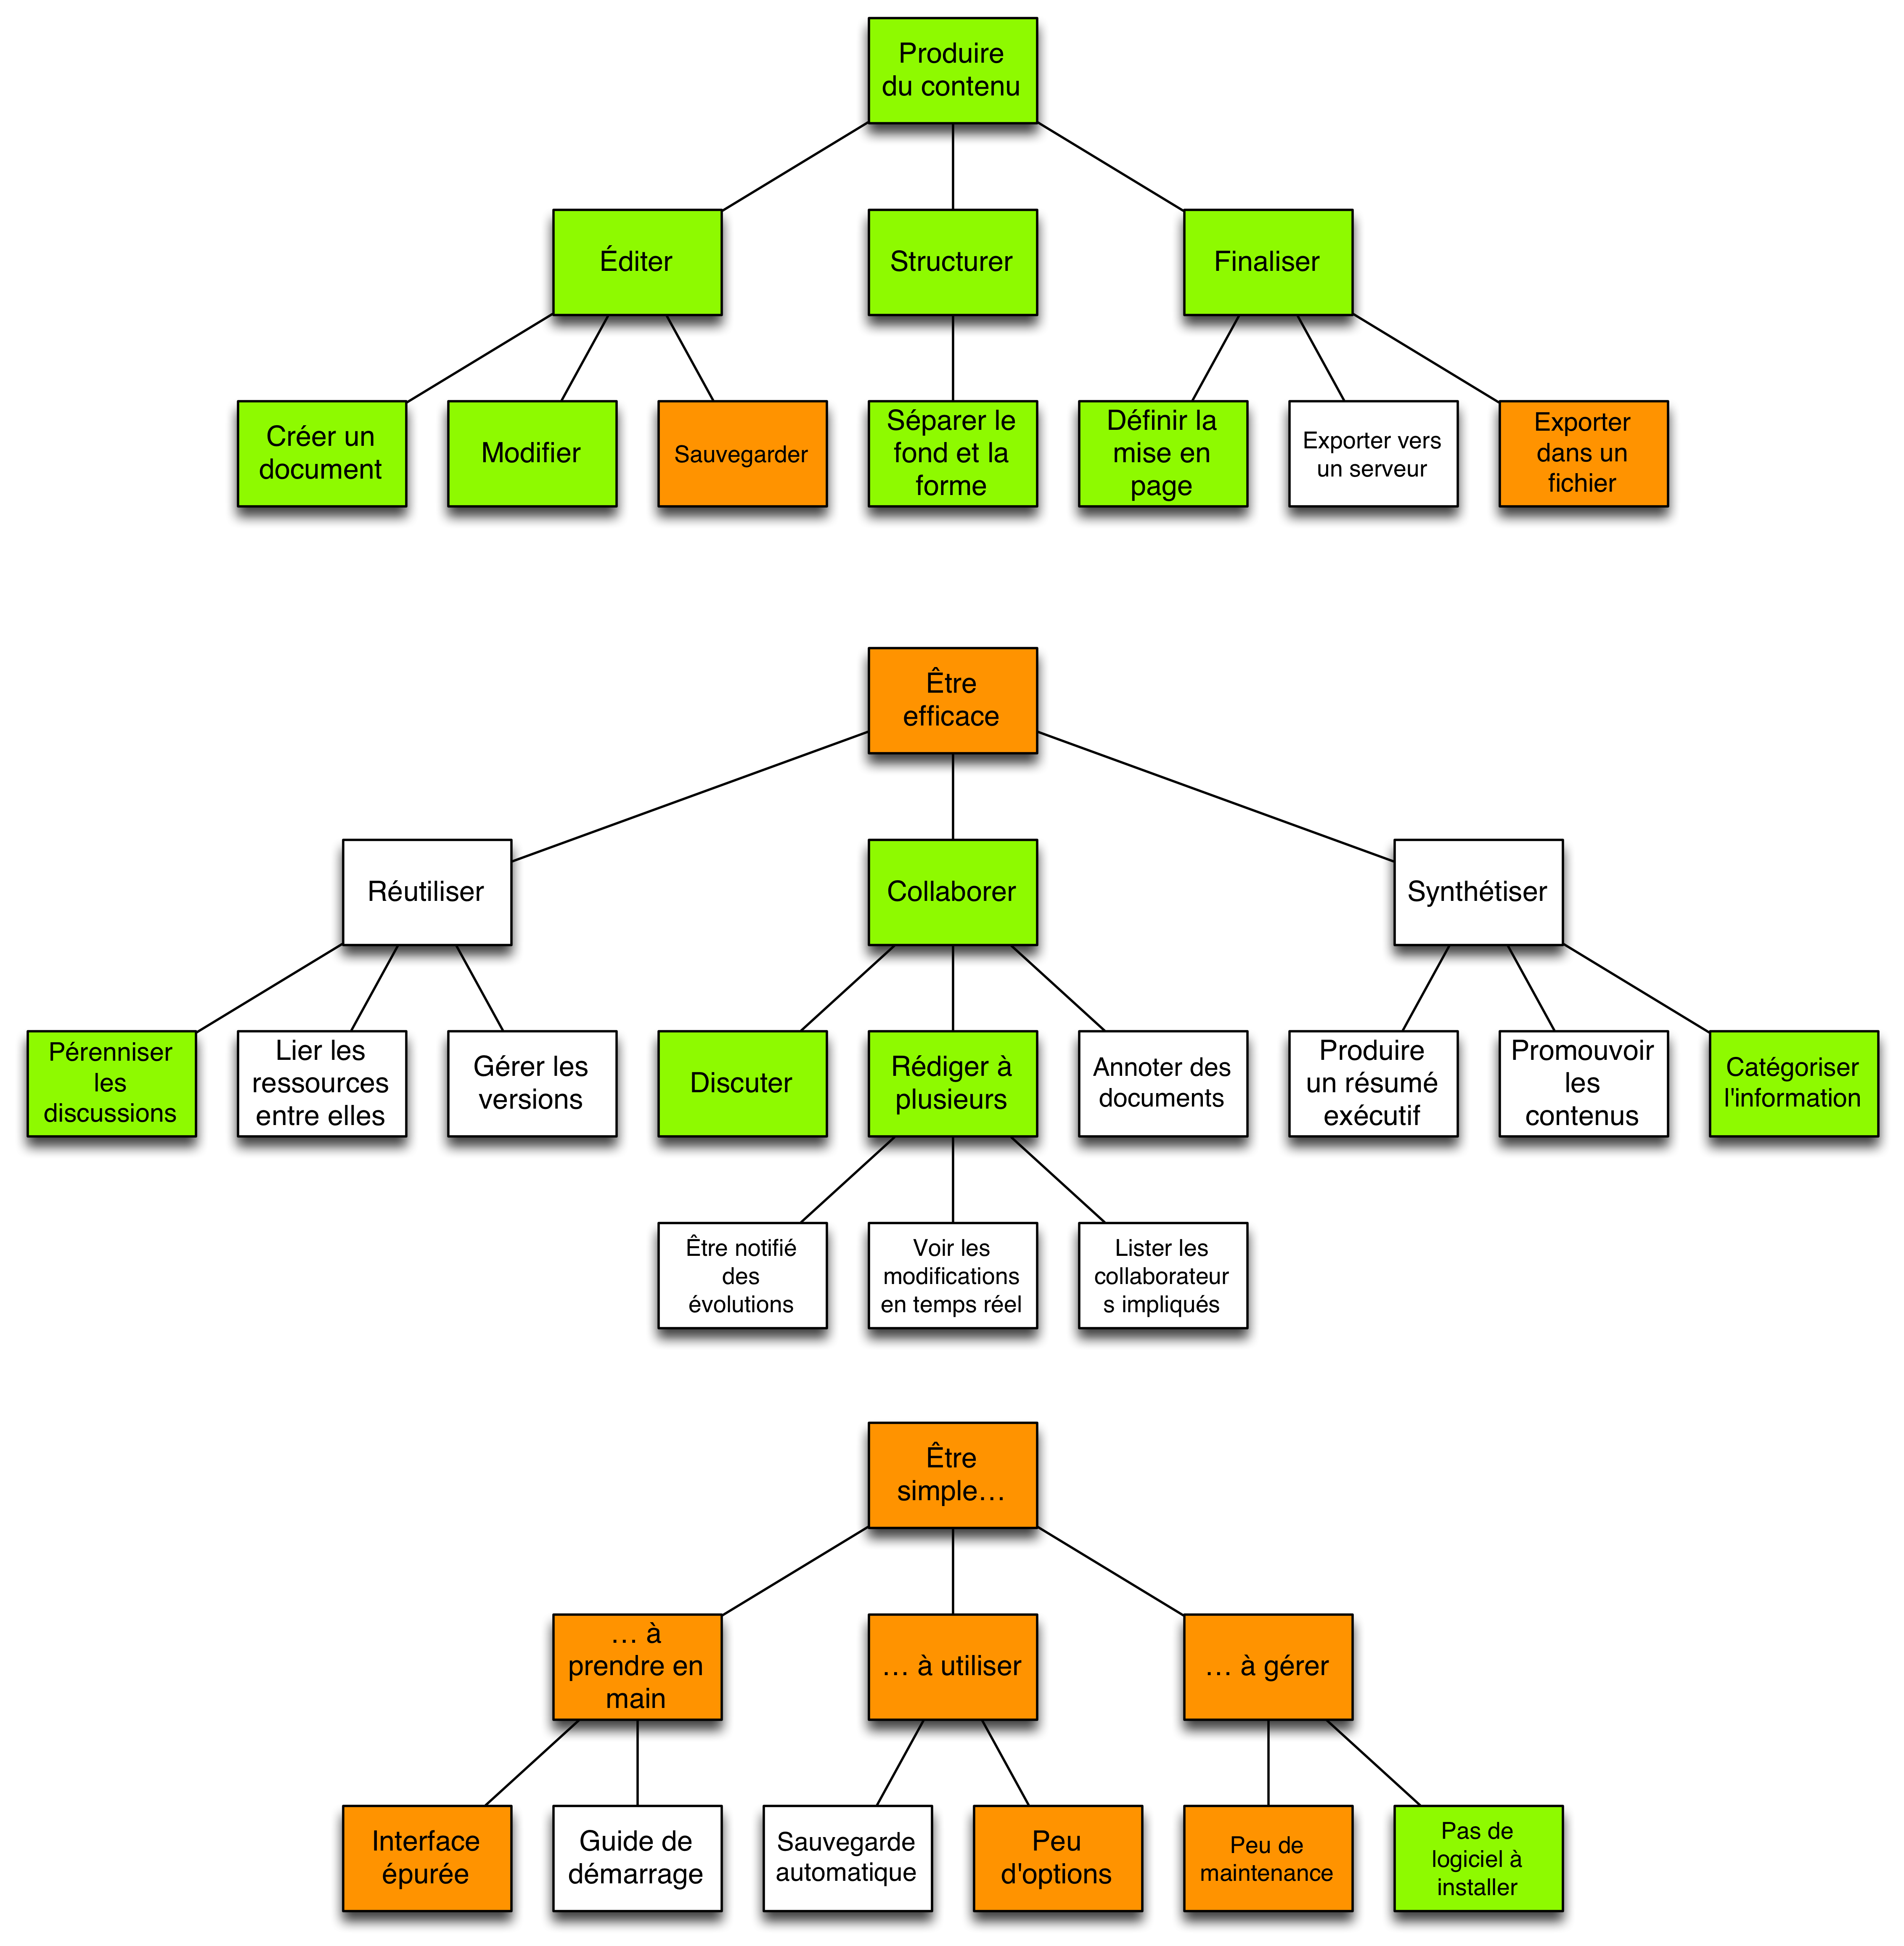
\includegraphics[width=\hsize]{analyse-fonctionnelle.png}
%\caption{Diagramme d'analyse fonctionnelle. Vert : fonction contrainte.
%Blanc : fonction complémentaire}
\end{figure}

Diagramme d'analyse fonctionnelle. Vert : fonction principale ; orange :
fonction contrainte ; blanc : fonction optionnelle.

\section{Description de la solution proposée}

Afin de pallier les problèmes soulevés dans la section précédente, nous
proposons un outil de rédaction collaborative de documents dont nous
allons désormais décrire les fonctionnalités.

\subsection{Rédaction}

Nous proposons avant tout un outil de rédaction et de production de
documents. Les utilisateurs pourront ainsi créer leurs propres documents
et les éditer, dans le but de produire un document final qui pourra être
exporté dans un format standard tel que le PDF. Il sera également
possible pour plusieurs collaborateurs d'éditer le même document en
temps réel.

Afin d'augmenter la productivité des utilisateurs, il nous semble
primordial de proposer un système permettant de séparer le fond et la
forme du document. Pour ce faire, nous proposons un outil d'édition des
styles parallèlement à la rédaction d'un document.

Il sera également possible d'intégrer des ressources externes telles que
des images ou des graphiques.

\subsection{Capitalisation sur les discussions}

Nous partons de l'observation suivante : \emph{les discussions et
critiques sont centrales à la rédaction d'un document}. Il est alors
impératif de ne pas séparer le document de son processus de rédaction.
Nous pouvons citer l'exemple du monde scientifique, où la relecture
d'articles de recherche occupe une part importante du métier de
chercheur et garantit la qualité des documents produits.

Quand une personne rédige un premier brouillon d'un document, elle va
demander l'avis de ses collaborateurs qui proposent leurs commentaires,
améliorant ainsi le document. Notre outil permet de \textbf{capitaliser
sur les discussions en les intégrant de manière forte aux documents}
auxquelles elles sont reliées. Un commentaire pourra alors être relié à
un paragraphe précis, permettant ainsi de le lire dans son contexte. Une
fois la discussion engagée, les différents participants pourront y
répondre en constituant un véritable fil de discussion centré autour
d'un paragraphe du document. Nous ajoutons à chaque fil de discussion la
possibilité d'en rédiger un \textbf{résumé}. Il complète la discussion
en proposant aux participants un court paragraphe résumant la discussion
et la décision prise par le groupe ; il permet ainsi aux lecteurs de
prendre connaissance de la décision finale sans avoir à lire le fil de
discussion entier. Une fois ce résumé rédigé, la conversation est figée
et ne peut évoluer.

L'ensemble des fils de discussions servira alors de base pour
l'amélioration et la création d'une nouvelle version du document. Au
cours de sa rédaction les différents résumés des discussions seront
affichés pour aider le rédacteur à prendre en compte les commentaires
des participants.

Chaque post et discussion aura un \emph{score d'importance}, calculé
automatiquement en fonction du nombre de réactions engendrées ou de
l'importance des participants. Cela nous permettra de \textbf{mettre en
avant les points de vue pertinents} afin d'aider les rédacteurs à
améliorer leurs documents.

Nous proposons également la possibilité de tenir une discussion
instantanée parmi les différents lecteurs d'un document, permettant
ainsi d'obtenir des retours rapides. Si la discussion instantanée est
jugée importante, elle pourra être \textbf{pérennisée} en étant
transformée en fil de discussion.

Ce principe de \textbf{rédaction itérative}, centrée sur un cycle de
rédaction et de discussion, a également l'avantage de conserver une
trace de l'évolution du document au cours du temps en maintenant un
historique des discussions importantes. Enfin, nous proposons un
\textbf{système de gestion de versions} : il sera possible de visualiser
les différences entre deux versions d'un même document, ainsi que les
discussions associées qui ont permis à ce document d'évoluer.

\subsection{Collaboration}

Comme précisé dans la section précédente, une organisation basée sur
l'e-mail comme outil de travail principal n'est pas optimale. Nous
proposons un outil où l'ensemble des participants sont organisés en
\textbf{communautés de travail}. Chaque participant peut faire partie de
plusieurs communautés de travail, qui peuvent alors s'apparenter aux
services des entreprises mais peuvent aussi regrouper des personnes aux
intérêts communs, telles qu'un groupe de travail transversal.

Fort de cette organisation, un utilisateur sera alors notifié de chaque
discussion se déroulant dans les communautés auxquelles il appartient.

Dans la même optique de collaboration, il est également possible
d'\textbf{inviter} une personne à une discussion ou de l'inviter à
relire un document afin de demander son opinion ou ses conseils. La
personne invitée peut alors lire le document et l'intégralité des
discussions associées.

Ces fonctionnalités de collaboration, de rédaction multi-utilisateurs
ainsi que de discussion contribuent ainsi à \textbf{améliorer
l'organisation des personnes} lors de leur travail.

\subsection{Inter-opérabilité}

Bien conscients de la nécessité de créer un outil utilisable avec les
systèmes déjà en place, nous proposons un ensemble de fonctionnalités
visant à intégrer notre outil dans l'écosystème logiciel existant.

Tout d'abord, l'ensemble des documents rédigés sont exportables dans un
format générique et standard tel que le PDF ou bien des formats
largement utilisés tels que le format Word. Cela permet aux personnes de
créer un fichier à partir d'un document créé dans notre outil.

Nous proposons également une intégration avec les e-mails. Le principe
est le suivant : à chaque publication de document, les personnes
recevront le PDF généré automatiquement par e-mail. Si elles répondent à
l'e-mail, le système ré-intègre la réponse dans l'outil en tant que
commentaire à propos du document. Ce système simple propose une
inter-opérabilité forte avec l'e-mail tout en permettant d'interagir de
manière aisée avec l'outil via un protocole standard. \# Description
technique Réaliser un outil tel que décrit précédemment nécessite
l'utilisation d'un ensemble de technologies logicielles ainsi qu'une
plate-forme matérielle gérant l'hébergement de la solution.

\begin{figure}[htbp]
\centering
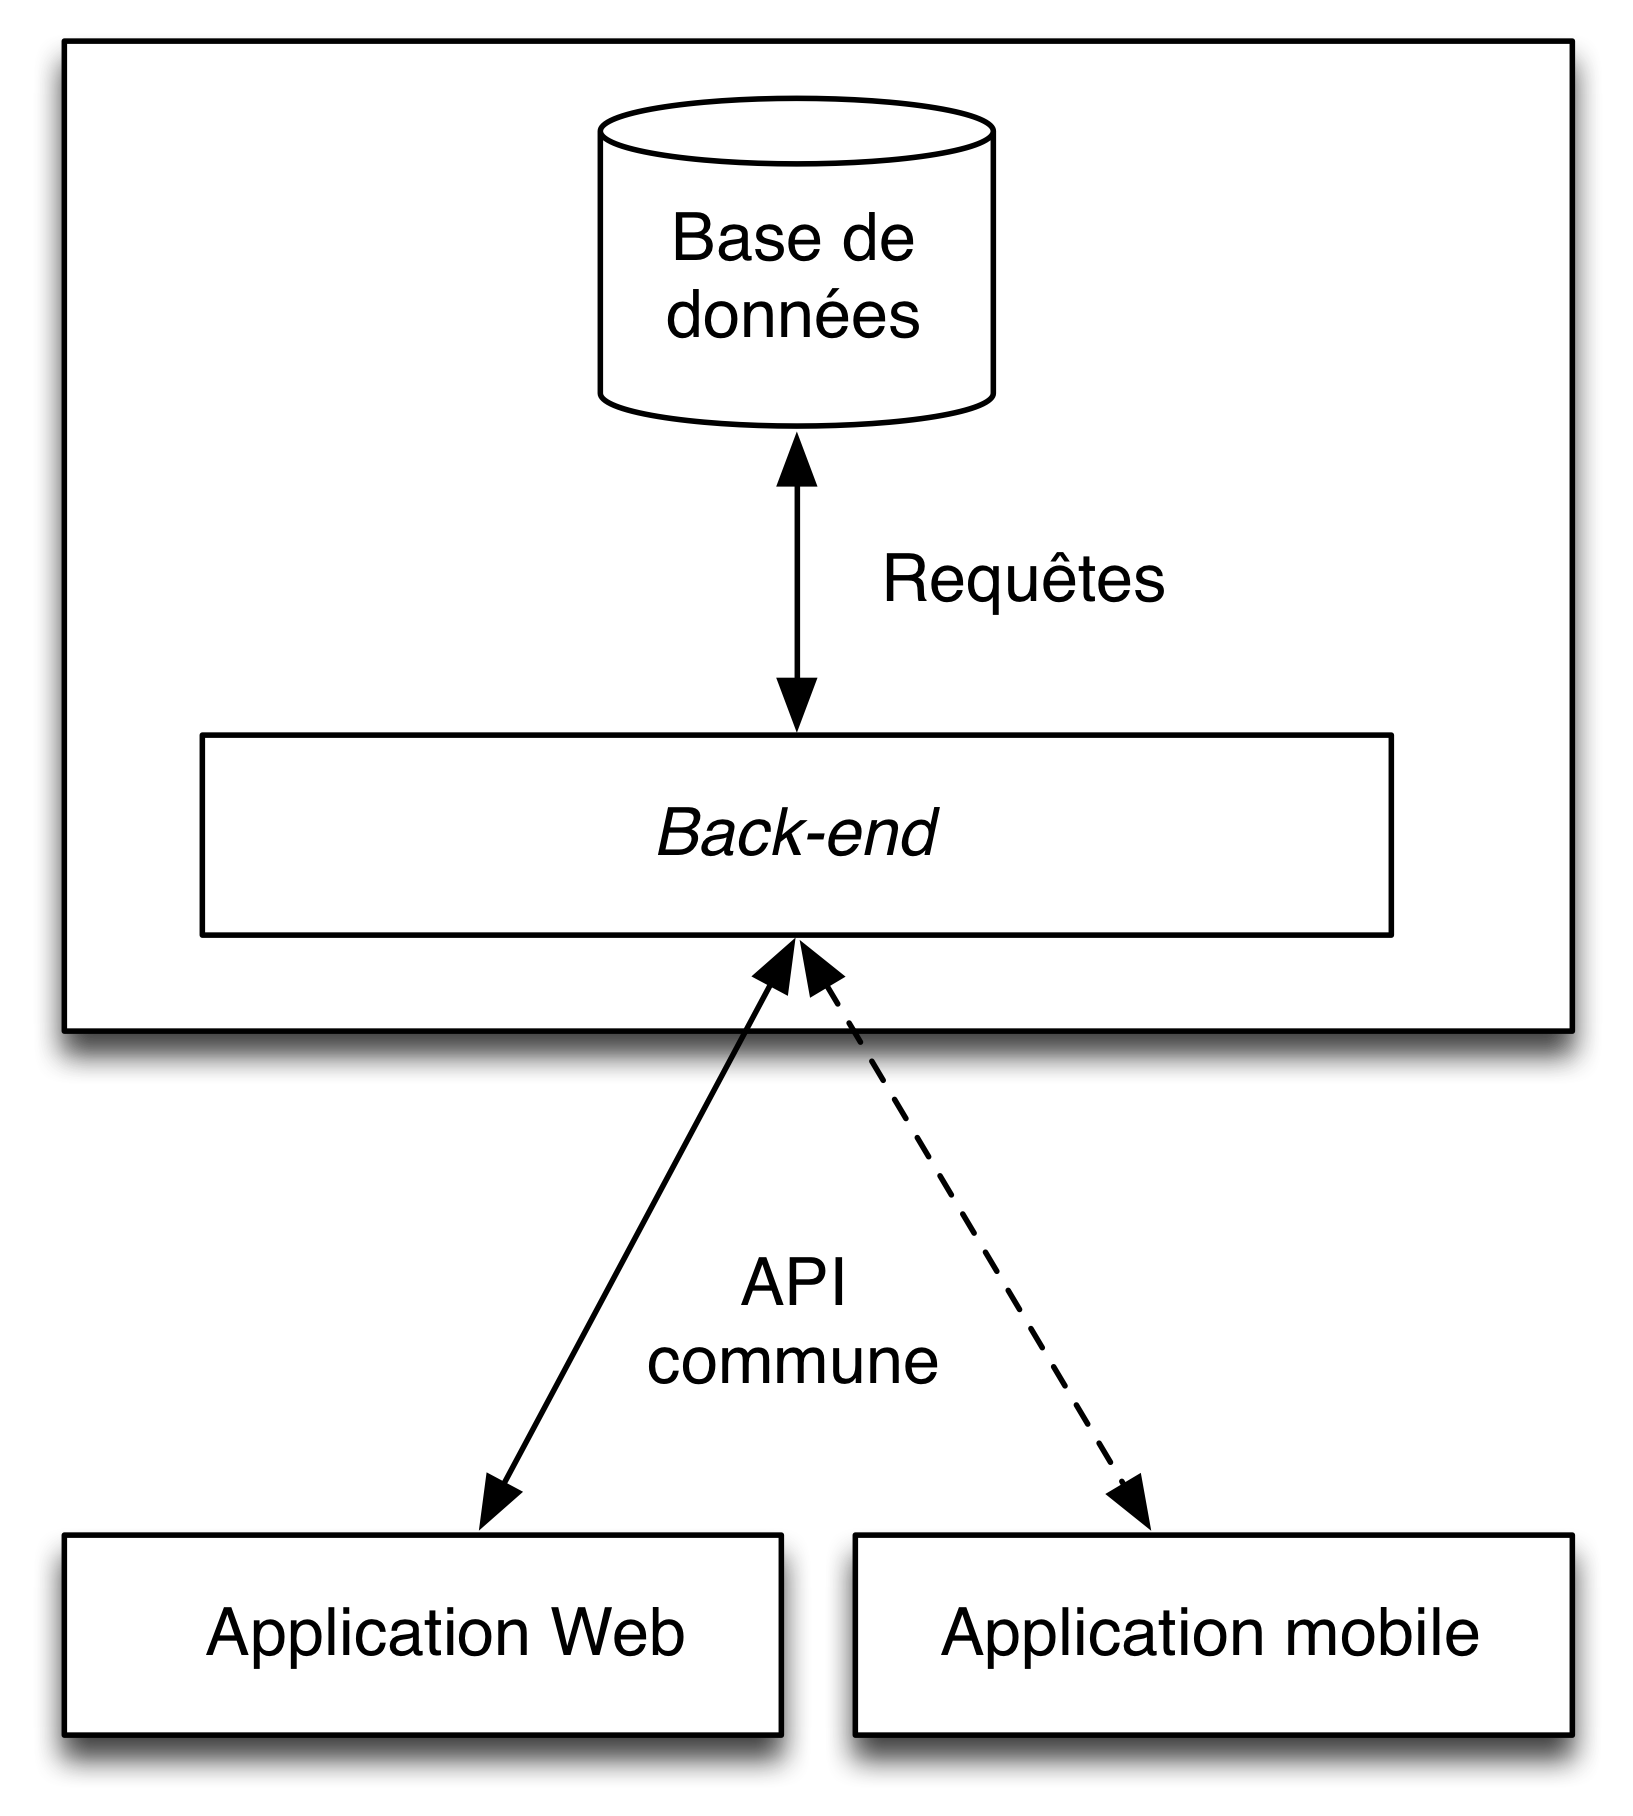
\includegraphics[width=\hsize]{architecture.png}
\end{figure}

Architecture choisie.

\subsection{Architecture logicielle}

Notre outil sera composé de deux parties principales : le
\emph{front-end} et le \emph{back-end}, basés intégralement sur des
technologies libres, accélérant ainsi notablement la conception de
l'outil tout en diminuant les coûts de développement.

Le \emph{front-end} est la partie visible par les utilisateurs.
Conformément à l'analyse fonctionnelle, il convient de proposer un outil
simple à gérer qui ne nécessite pas de logiciel à installer. Nous
proposons ainsi un outil accessible via une interface Web, ce qui permet
à l'utilisateur de s'affranchir des contraintes d'installation. De plus,
ce mode de fonctionnement permet une mise à jour transparente de
l'application : il suffit que les utilisateurs visitent le site pour
utiliser la dernière version de l'outil sans action particulière de leur
part. On notera de plus qu'une application Web est \emph{de facto}
compatible avec tous les systèmes d'exploitation existants. Afin
d'accélérer le développement nous utiliserons des technologies basées
sur JavaScript et HTML5 pour construire l'interface. D'un point de vue
expérience utilisateur, l'utilisation de langages clients tels que
JavaScript permet la création d'interfaces très réactives et
interactives. Il n'est pas exclu de créer une application mobile en tant
que deuxième \emph{front-end} mais cela ne constitue pas la priorité du
développement.

Le \emph{back-end} est la partie invisible par les utilisateurs et est
composé de deux parties. Avant tout, il doit stocker toutes les données
de l'application telles que les informations associées aux utilisateurs,
leurs conversations et leurs documents. Cette fonction sera assurée par
un système de gestion de bases de données. Le \emph{back-end} devra
également comporter une couche logicielle permettant au \emph{front-end}
d'acquérir et de mettre à jour les données tout en respectant les règles
de sécurité et les autorisations accordées aux utilisateurs.

\subsection{Architecture matérielle}

Comme soulevé dans l'analyse fonctionnelle, il convient de mettre à la
disposition des utilisateurs un système simple à mettre en place et à
gérer. Dans cette optique, nous proposerons une structure d'hébergement
payante de l'application - détaillée dans la partie marketing de ce
document - afin qu'ils n'aient pas à se soucier de cette contrainte.

Dans le but de permettre une flexibilité maximale, nous utiliserons un
hébergement de type \emph{cloud IaaS}. Ces hébergements supportent une
montée en charge rapide en cas de pic d'utilisation en permettant
d'augmenter la puissance de calcul ou de stockage à la demande.
Stratégiquement, ils permettent à l'équipe de se concentrer sur le
développement de l'application et de passer le minimum de temps sur son
implantation, car l'hébergeur prend en charge toutes les considérations
matérielles. De plus, utiliser une architecture \emph{Infrastructure as
a Service} ne nous limitera pas quant aux solutions techniques utilisées
pour construire notre produit. \# Étude du marché

Le monde d'aujourd'hui est de plus en plus marqué par l'évolution des
méthodes de travail résultant de l'essor des technologies. Cette
évolution tend à mener vers un travail de plus en plus collaboratif. Le
travailleur solitaire n'a plus sa place dans le monde globalisé qui est
le nôtre. Un bon travail d'équipe est devenu essentiel pour surmonter la
concurrence planétaire, d'où l'apparition de nombreux outils de travail
collaboratif. Ces outils visent à améliorer la communication au sein
d'un groupe de travail.

De par nature l'homme transmet ce qu'il sait en le communiquant. De nos
jours, il utilise la technologie afin non seulement de partager son
savoir mais également de le pérenniser et de l'enrichir par une mise en
commun des connaissances mondiales.

Le \textbf{travail collaboratif} peut être défini comme un mode de
travail non hiérarchisé dans lequel des personnes mettent en commun leur
créativité et leurs compétences afin d'atteindre un même objectif.
Aujourd'hui, les travaux en collaboration s'appuient de plus en plus sur
les technologies de l'information et de la communication. Les nouveaux
outils permettent d'optimiser l'efficacité d'un groupe de personnes
travaillant ensemble sur des projets même si elles sont très dispersées
dans l'espace et le temps. Les domaines suivants nécessitent fortement
de tels outils :

\begin{itemize}
\itemsep1pt\parskip0pt\parsep0pt
\item
  \textbf{Gestion documentaire} pour harmoniser le travail sur
  différentes versions de documents
\item
  \textbf{Gestion de projet} pour manager le déroulement d'un projet
\item
  \textbf{Gestion des relations sociales} pour valoriser les relations
  internes et externes à une organisation
\item
  \textbf{Gestion des connaissances} pour capitaliser les savoirs et
  mieux partager les informations
\end{itemize}

\subsection{Comportements du marché}

Chaque utilisateur du Web utilise aujourd'hui des outils de travail
collaboratif divers et variés. Certains proposent un moyen direct de
communication : par téléphone, par messagerie instantanée, par vidéo
conférence\ldots{} D'autres moyens sont eux asynchrones : e-mail, SMS,
forums\ldots{} Selon l'INSEE, 45\% des sociétés françaises étaient
dotées d'un intranet début 2010. De plus, concernant le travail
collaboratif sur un même produit amené à beaucoup évoluer dans le temps,
on remarque l'utilisation d'outils permettant le versioning et le
partage de documents. Il est également intéressant de noter que certains
outils qui à l'origine n'étaient pas destinés à faciliter le travail
collaboratif ont évolué en ce sens. Par exemple, Facebook est devenu un
organisateur d'événement.

\subsection{Étude de l'environnement}

\subsubsection{Intranet}

Les entreprises maintiennent aujourd'hui majoritairement un intranet. Ce
dernier leur permet de partager des documents et toutes sortes de
ressources informatiques. Ces activités nécessitent un investissement
humain et financier lourd, souvent disproportionné - pour les PME et
associations - par rapport à la criticité de ces outils dans les
activités cœur de l'entreprise. Ce marché représentait en 2010 environ
289\euro{} par an et par entreprise en moyenne pour les grands
groupes ; c'est donc dans une optique de rationalisation des coûts que
nous nous positionnons en déchargeant les petites et moyennes structures
de cette responsabilité.

\subsubsection{Traitement de texte}

Les logiciels de traitement de texte sont un outil plébiscité par les
entreprises qui en sont universellement clientes et utilisatrices. En
effet, il est constamment nécessaire pour elles de rédiger et mettre en
forme de l'information dans leur activité quotidienne. Un acteur possède
une position dominante sur ce marché : Microsoft Business, avec sa suite
Office et son logiciel phare Word. Cette division génère 20 milliards
d'euros de chiffre d'affaires par an, soit un tiers du chiffre
d'affaires total de Microsoft. C'est aussi 500 millions d'utilisateurs à
travers le monde pour un prix public de 269\euro{} par licence (petites
entreprises) à 539\euro{} par licence (professionnel). Une autre offre a
fait son apparition en 2011, Microsoft Office 365, qui est proposé en
mode \emph{SaaS} - abonnement mensuel - pour un prix de 4,80\euro{} à
19\euro{} par mois selon les services intégrés - messagerie
électronique, visualisation et édition en ligne, stockage dans le cloud,
collaboration, voix sur IP, etc.

\subsubsection{Nouveaux concepts émergents}

Il est intéressant de remarquer l'émergence de nouveaux modes de
collaboration, qui soulignent bien notre entrée dans l'ère du travail a
plusieurs. Le \emph{coworking}, par exemple, est un nouveau terme
désignant un type d'organisation du travail qui regroupe deux notions :
un espace de travail partagé, mais aussi un réseau de travailleurs
encourageant l'échange et l'ouverture. Similaires aux \emph{cafés
philos}, ces espaces publics de travail sont de plus en plus nombreux à
apparaître dans les grandes villes du monde et souligne un désir de
collaboration de plus en plus fort dans le monde du travail. La notion
de \emph{crowdsourcing} désigne quant à elle une pratique consistant à
réunir un grand groupe de personnes intéréssées par un même sujet avec
pour but de trouver une solution à un problème. Par exemple,
\textbf{Amazon Mechanical Turk} (MTurk) est un marché internet de
\emph{crowdsourcing} permettant à des programmeurs de coordonner des
travaux non réalisables par des machines. On trouve en ligne diverses
tâches que quiconque peut réaliser. Celles-ci sont variées et proposent
en retour une petite rénumération. Ces tâches peuvent par exemple être
une sélection de photos pour une publicité ou une traduction en anglais
de tweets écrit dans un dialecte rare. En janvier 2011, MTurk recensait
500.000 travailleurs de 190 pays différents.

Un sondage réalisé auprès de 113 personnes nous a permis de mettre en
évidence la grande variété d'outils utilisés pour les travaux
collaboratifs.

\begin{figure}[htbp]
\centering
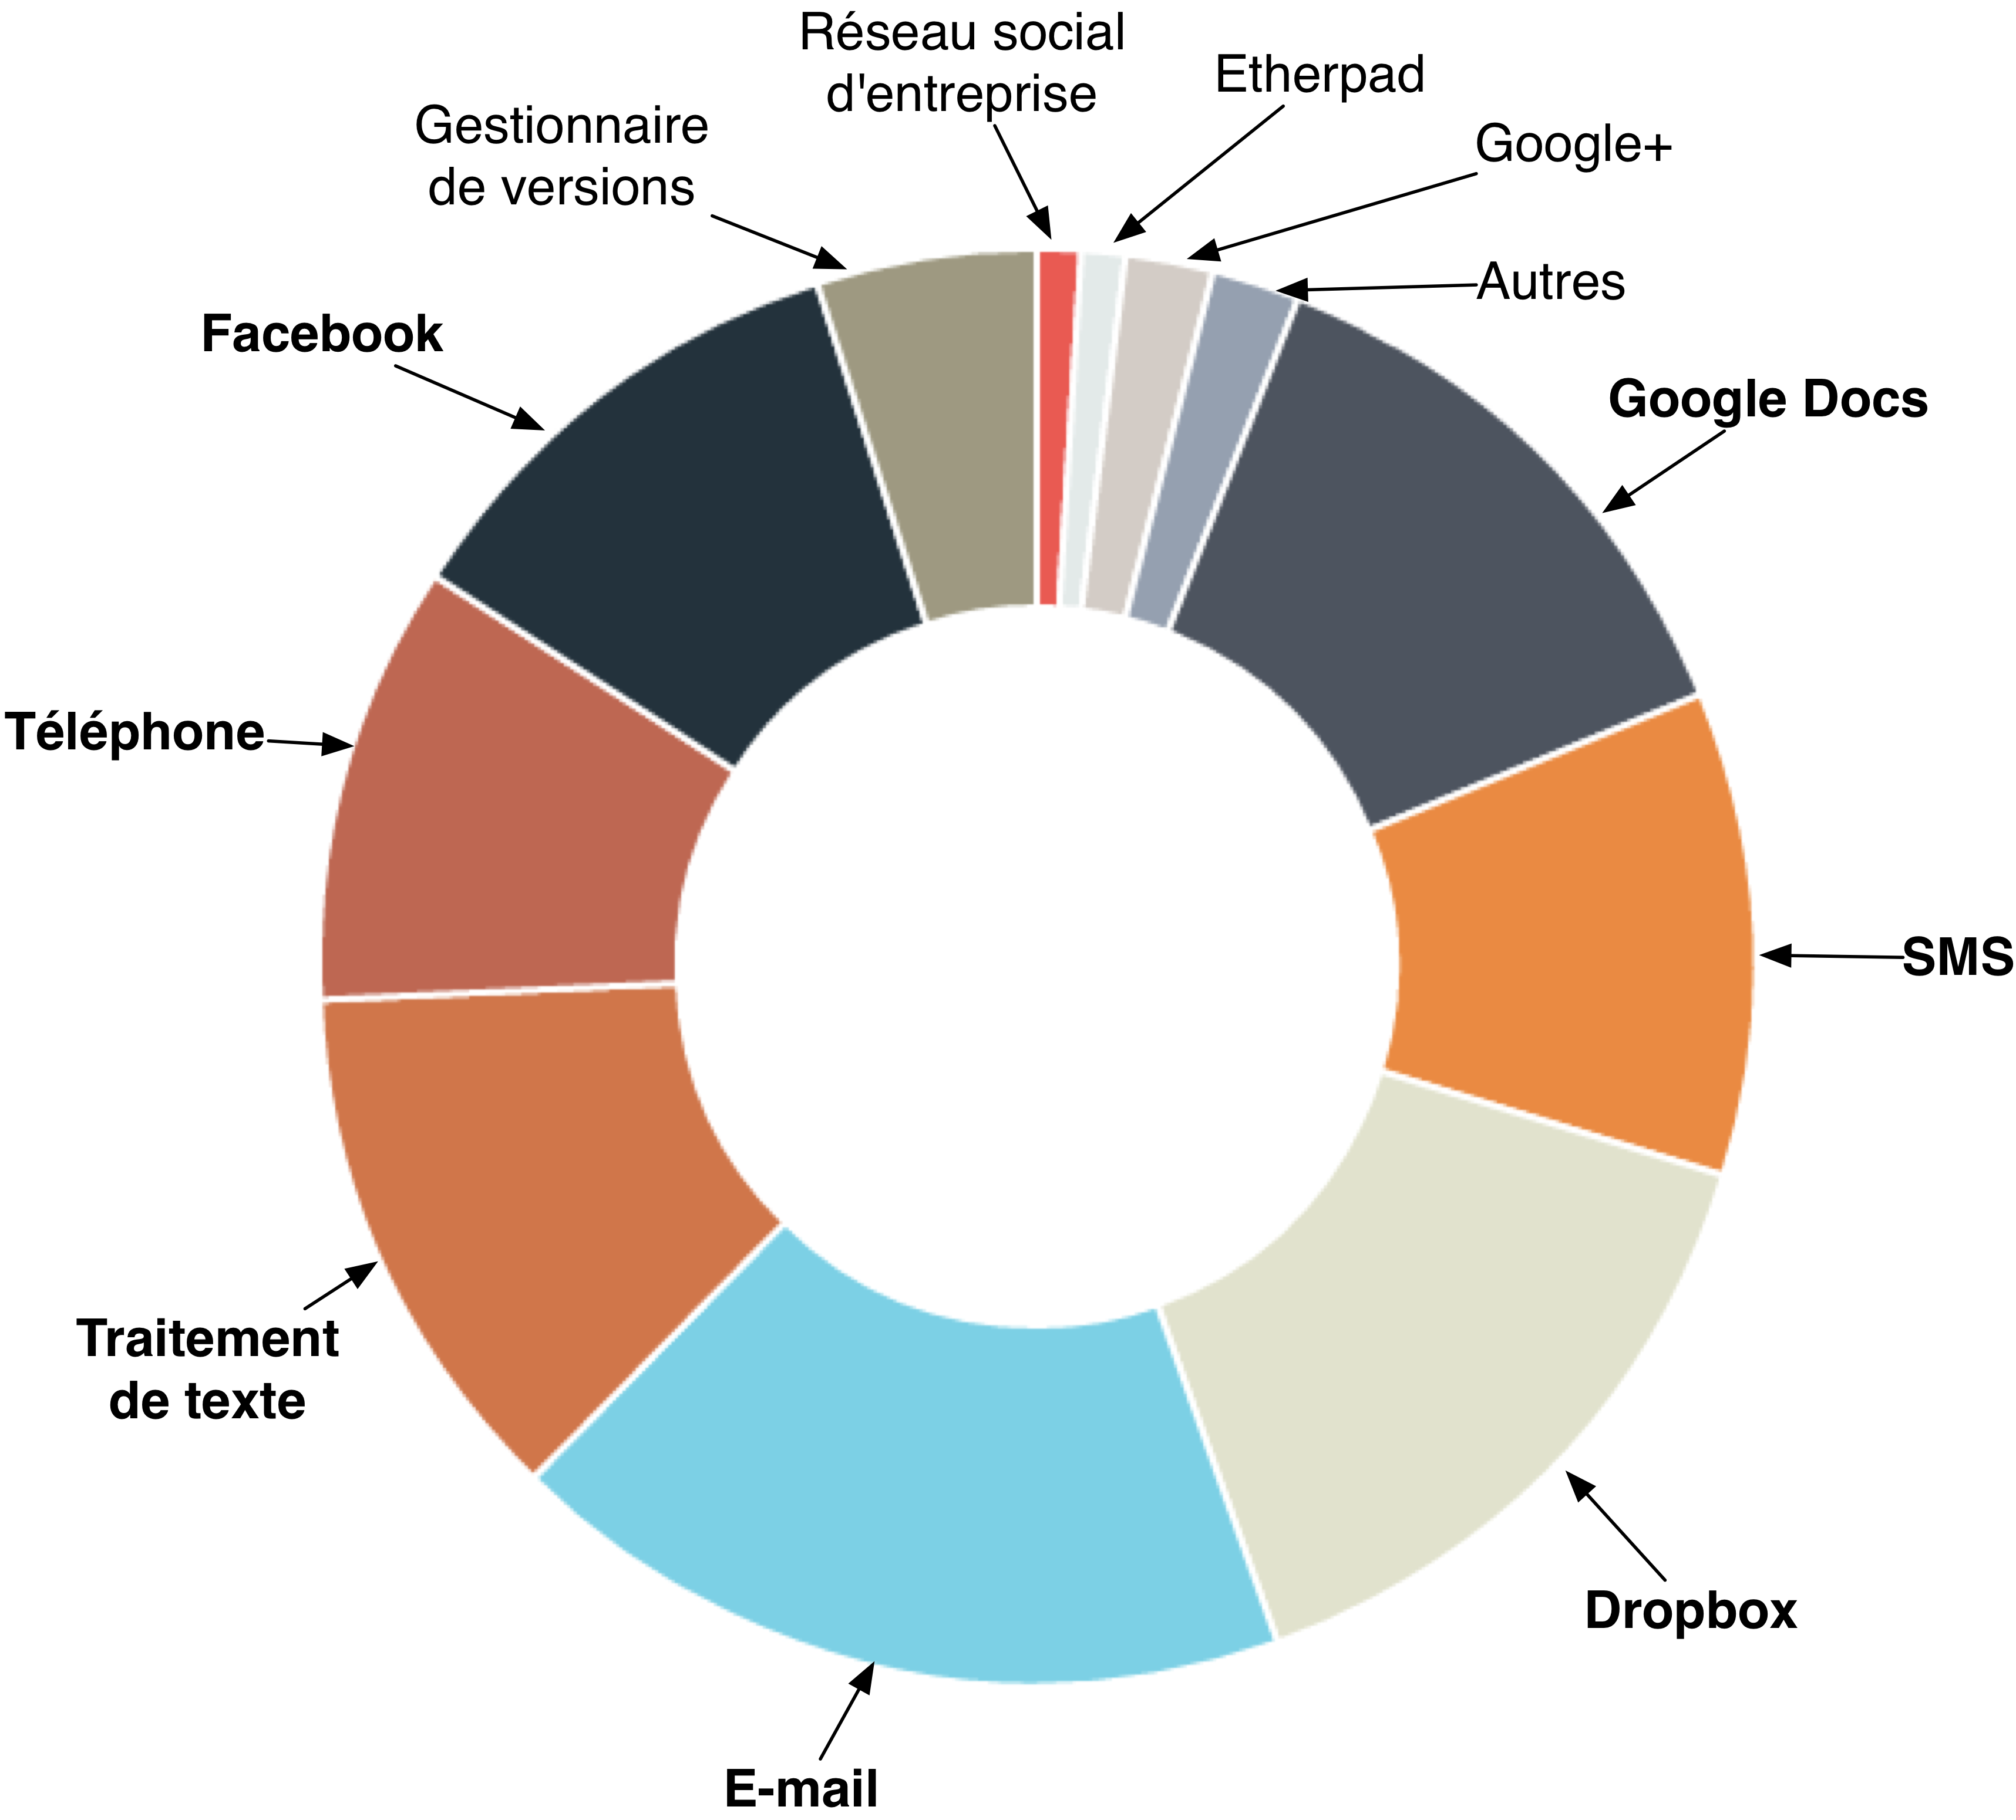
\includegraphics[width=\hsize]{sondageOutils.png}
\caption{Sondage : quels outils de collaborations utilisez vous ?}
\end{figure}

Ce résultat montre la diversité des outils utilisés. Il ressort que
l'e-mail, Dropbox et Google Docs constituent les moyens principaux de
collaboration.

Nous analysons maintenant les grandes catégories d'outils de travail
collaboratif.

\subsubsection{Gestionnaires de versionning et outils de partage de
documents}

Ils sont en place sur le marché depuis quelques années déjà, comme le
montre la forte implantation en entreprise de IBM Lotus Notes depuis
plus de 20 ans. En revanche, l'ouverture au grand public est plus
récente. Dropbox est un des exemples connus car il a su s'imposer dans
les entreprises, mais également chez l'utilisateur \emph{lambda} en
démystifiant la complexité inhérente au partage. Comme leur blog
l'indique, cet outil est utilisé par les professionnels de plus de 2
millions d'entreprises et par les particuliers avec plus de 50 millions
de comptes ouverts depuis 2007.

On pourra également noter que l'aspect social a pris de l'importance.
Par exemple, Github et Microsoft Sharepoint proposent une page de profil
présentant rapidement l'identité de l'utilisateur et les projets
auxquels il a contribué. L'interaction entre les divers utilisateurs est
de plus en plus mise en avant afin de les rapprocher en raison d'un
intérêt commun.

Le succès rencontré est fulgurant, comme le montre le graphique suivant
représentant l'évolution du nombre de dépôts Github au cours de ces
dernières années :

\begin{figure}[htbp]
\centering
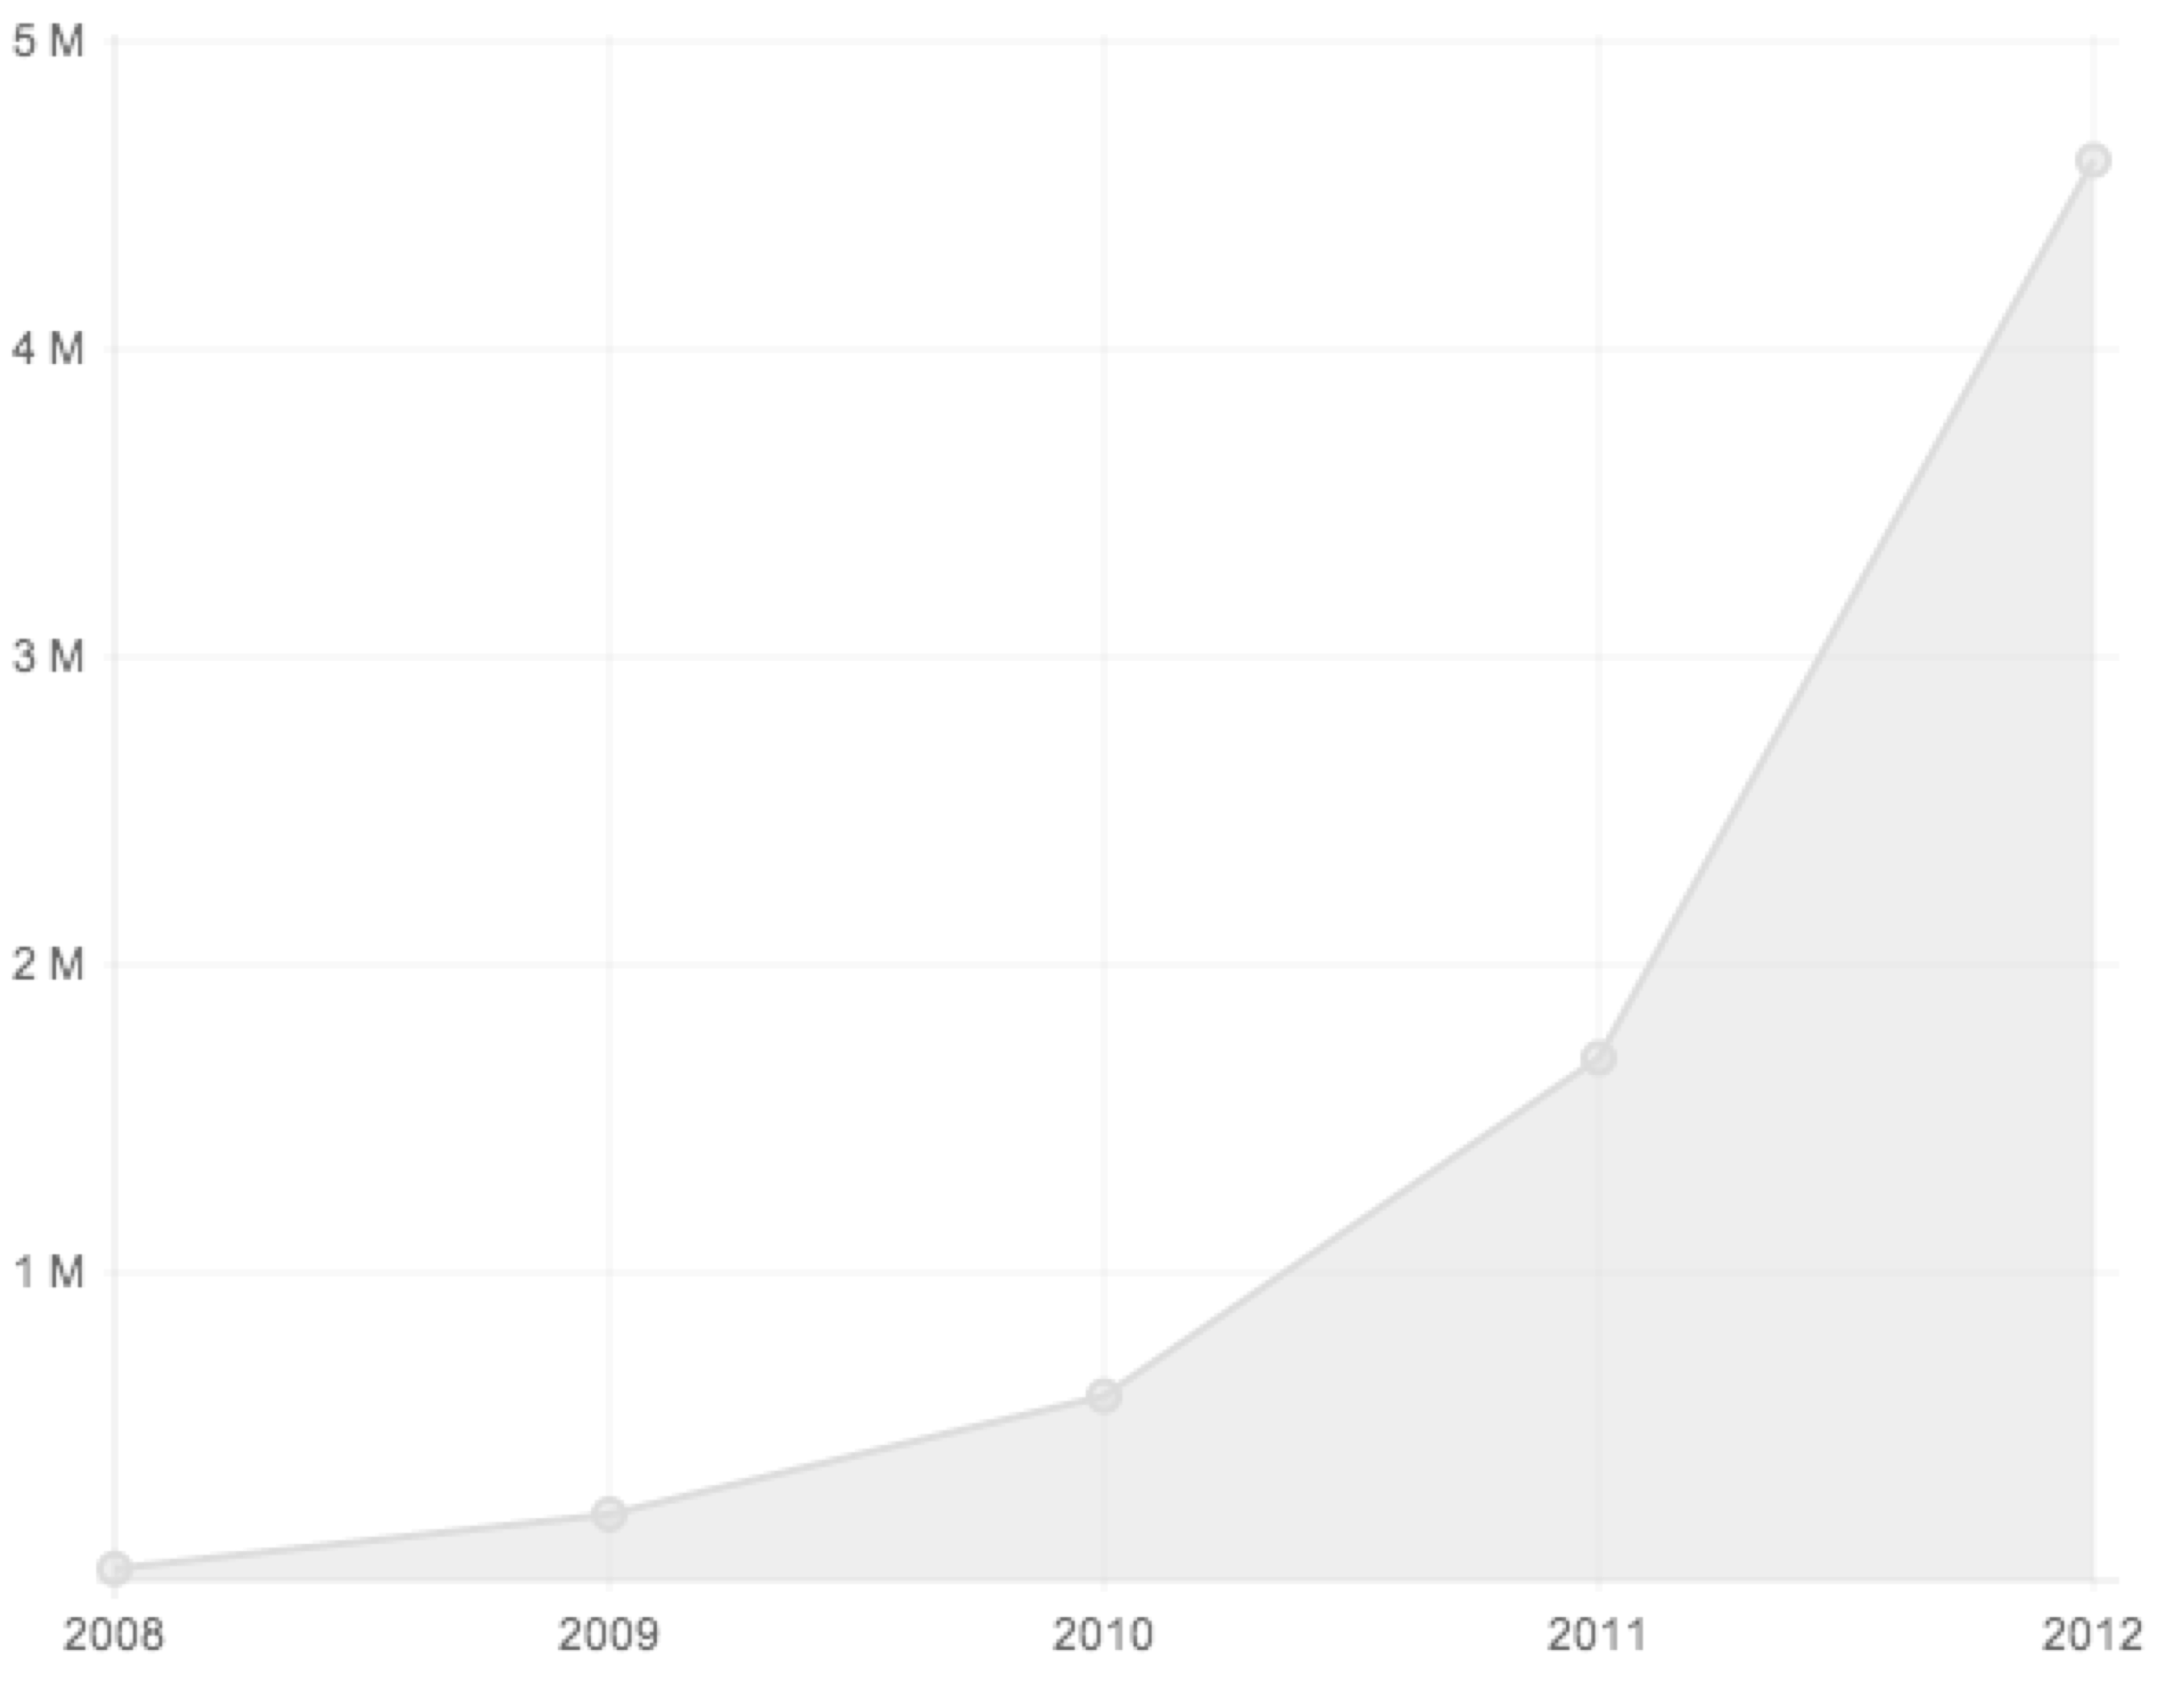
\includegraphics[width=\hsize]{githubEvolutionDepot.png}
\caption{évolution du nombre de dépôt sur Github}
\end{figure}

\subsubsection{Éditeurs collaboratifs}

Ces outils se concentrent sur l'édition de documents en groupe visant à
partager des savoirs et capitaliser sur ces derniers. On distingue deux
catégories d'outils :

\begin{itemize}
\itemsep1pt\parskip0pt\parsep0pt
\item
  Les outils fonctionnant en temps réel tels que Google Docs et
  EtherPad, qui sont de plus en plus utilisés par les entreprises
\item
  Les outils asynchrones, comme Wikipédia qui compte aujourd'hui 18,5
  millions d'utilisateurs et qui a permis de générer environ 29 millions
  de pages wiki en travail collaboratif
\end{itemize}

Les trois outils mentionnés ci-dessus constituent nos principaux
concurrents. Cependant, notre sondage a mis en évidence le désir d'une
amélioration dans ce domaine.

\emph{Avec les outils actuels, vous estimez que l'édition collaborative
de documents est :}

\begin{figure}[htbp]
\centering
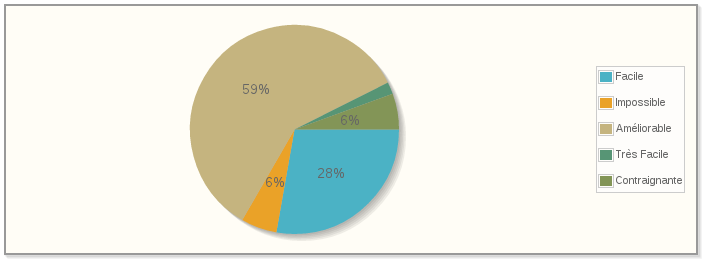
\includegraphics[width=\hsize]{sondageOpigionsOutilsActuels.png}
\caption{Sondage : qualité de l'édition collaborative ?}
\end{figure}

\emph{Seriez-vous intéressé par un nouvel outil permettant de faciliter
la rédaction de documents en groupe ?}

\begin{figure}[htbp]
\centering
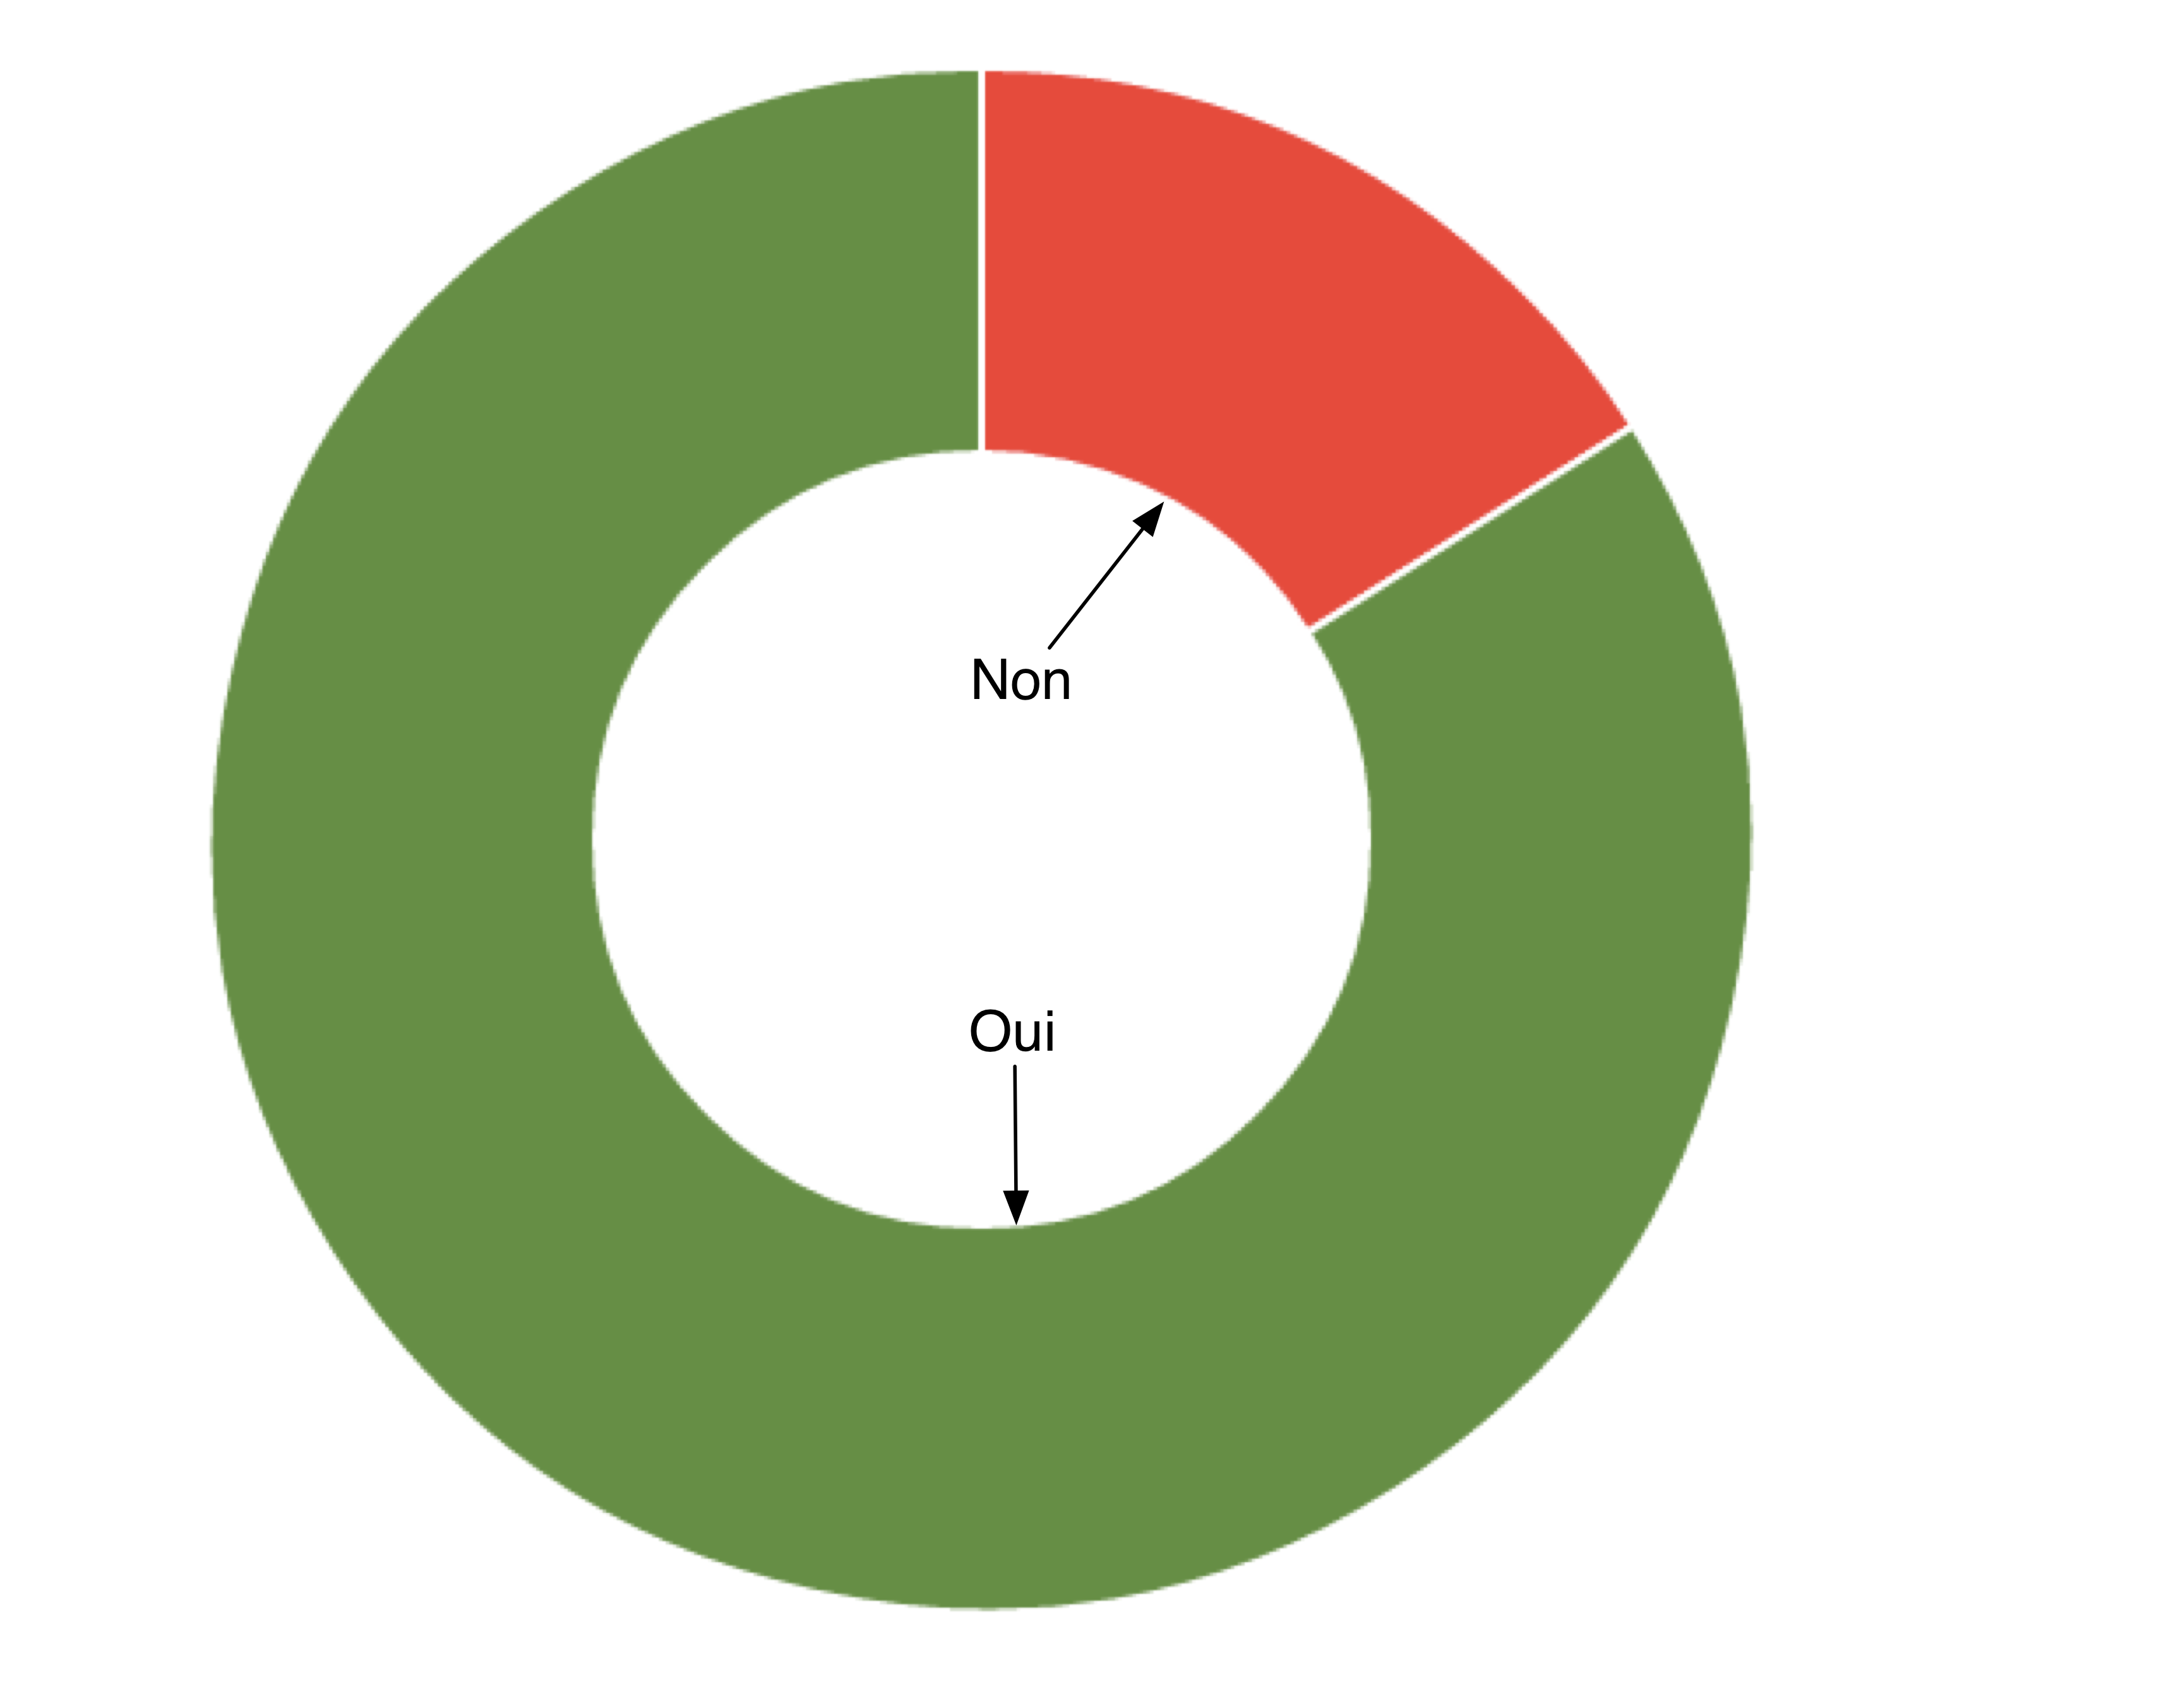
\includegraphics[width=\hsize]{sondageBesoins.png}
\caption{Sondage : besoin d'un nouvel outil ?}
\end{figure}

Nous avons également profité de ce sondage pour mettre en évidence les
formats d'exportation les plus attendu par le public.

\begin{figure}[htbp]
\centering
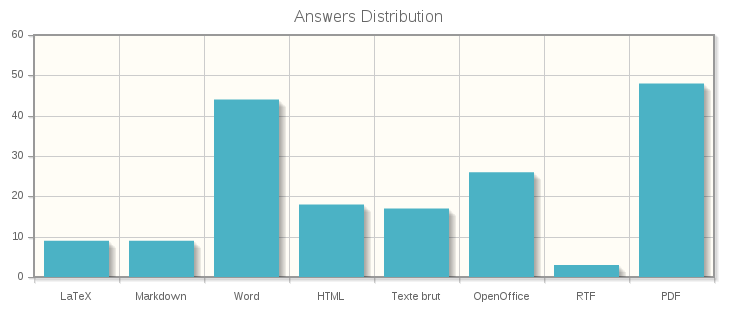
\includegraphics[width=\hsize]{sondageFormats.png}
\caption{Sondage : formats les plus important}
\end{figure}

\subsection{Opportunités de lancement}

\subsubsection{Points sensibles}

Comme montré ci-dessus, il y a beaucoup de concurrents potentiels et ils
sont d'envergures. De plus, la migration sur notre outil peut être
difficile pour les sociétés dont les employés peuvent être réfractaires
au changement. Enfin, notre outil, tout comme une communauté, prend
d'autant plus de valeur que son nombre d'utilisateurs est grand. Le
décollage de ce dernier peut donc être un peu fastidieux au départ.

\subsubsection{Points forts}

Pouvoir pérenniser les discussions et utiliser différents supports sur
un même outil est une idée innovante qui, suite à notre étude de marché,
nous semble répondre à un besoin réel. Notre objectif est de faire
ressortir les informations de valeur, ce qui est un point crucial de nos
jours.

On parle également aujourd'hui du "Web 3.0" ou du "Web sémantique"
dont le but principal viserait à orienter l'évolution du Web pour
permettre aux utilisateurs sans intermédiaire de trouver, partager et
combiner l'information plus facilement. C'est dans cette direction que
notre outil veut servir ses utilisateurs.

Dans la culture de l'internet on parle de la "loi des 1 pourcent" ou
du "principe 90-9-1" qui gouverne l'apport d'informations sur la
toile. Celle-ci stipule que seul 1 pourcent des utilisateurs du Web
contribuent à créer de l'information, 9 pourcents contribuent par leurs
remarques et leurs commentaires à la bonification de cette information
et que les 90 restants ne font que profiter de l'information créée mais
sans en créer eux-mêmes. Notre outil aurait pour but de donner plus de
pouvoir aux créateurs et de faciliter la contribution à la création
d'information en ligne afin d'amener les personnes à mieux et plus
produire ensemble !

\begin{figure}[htbp]
\centering
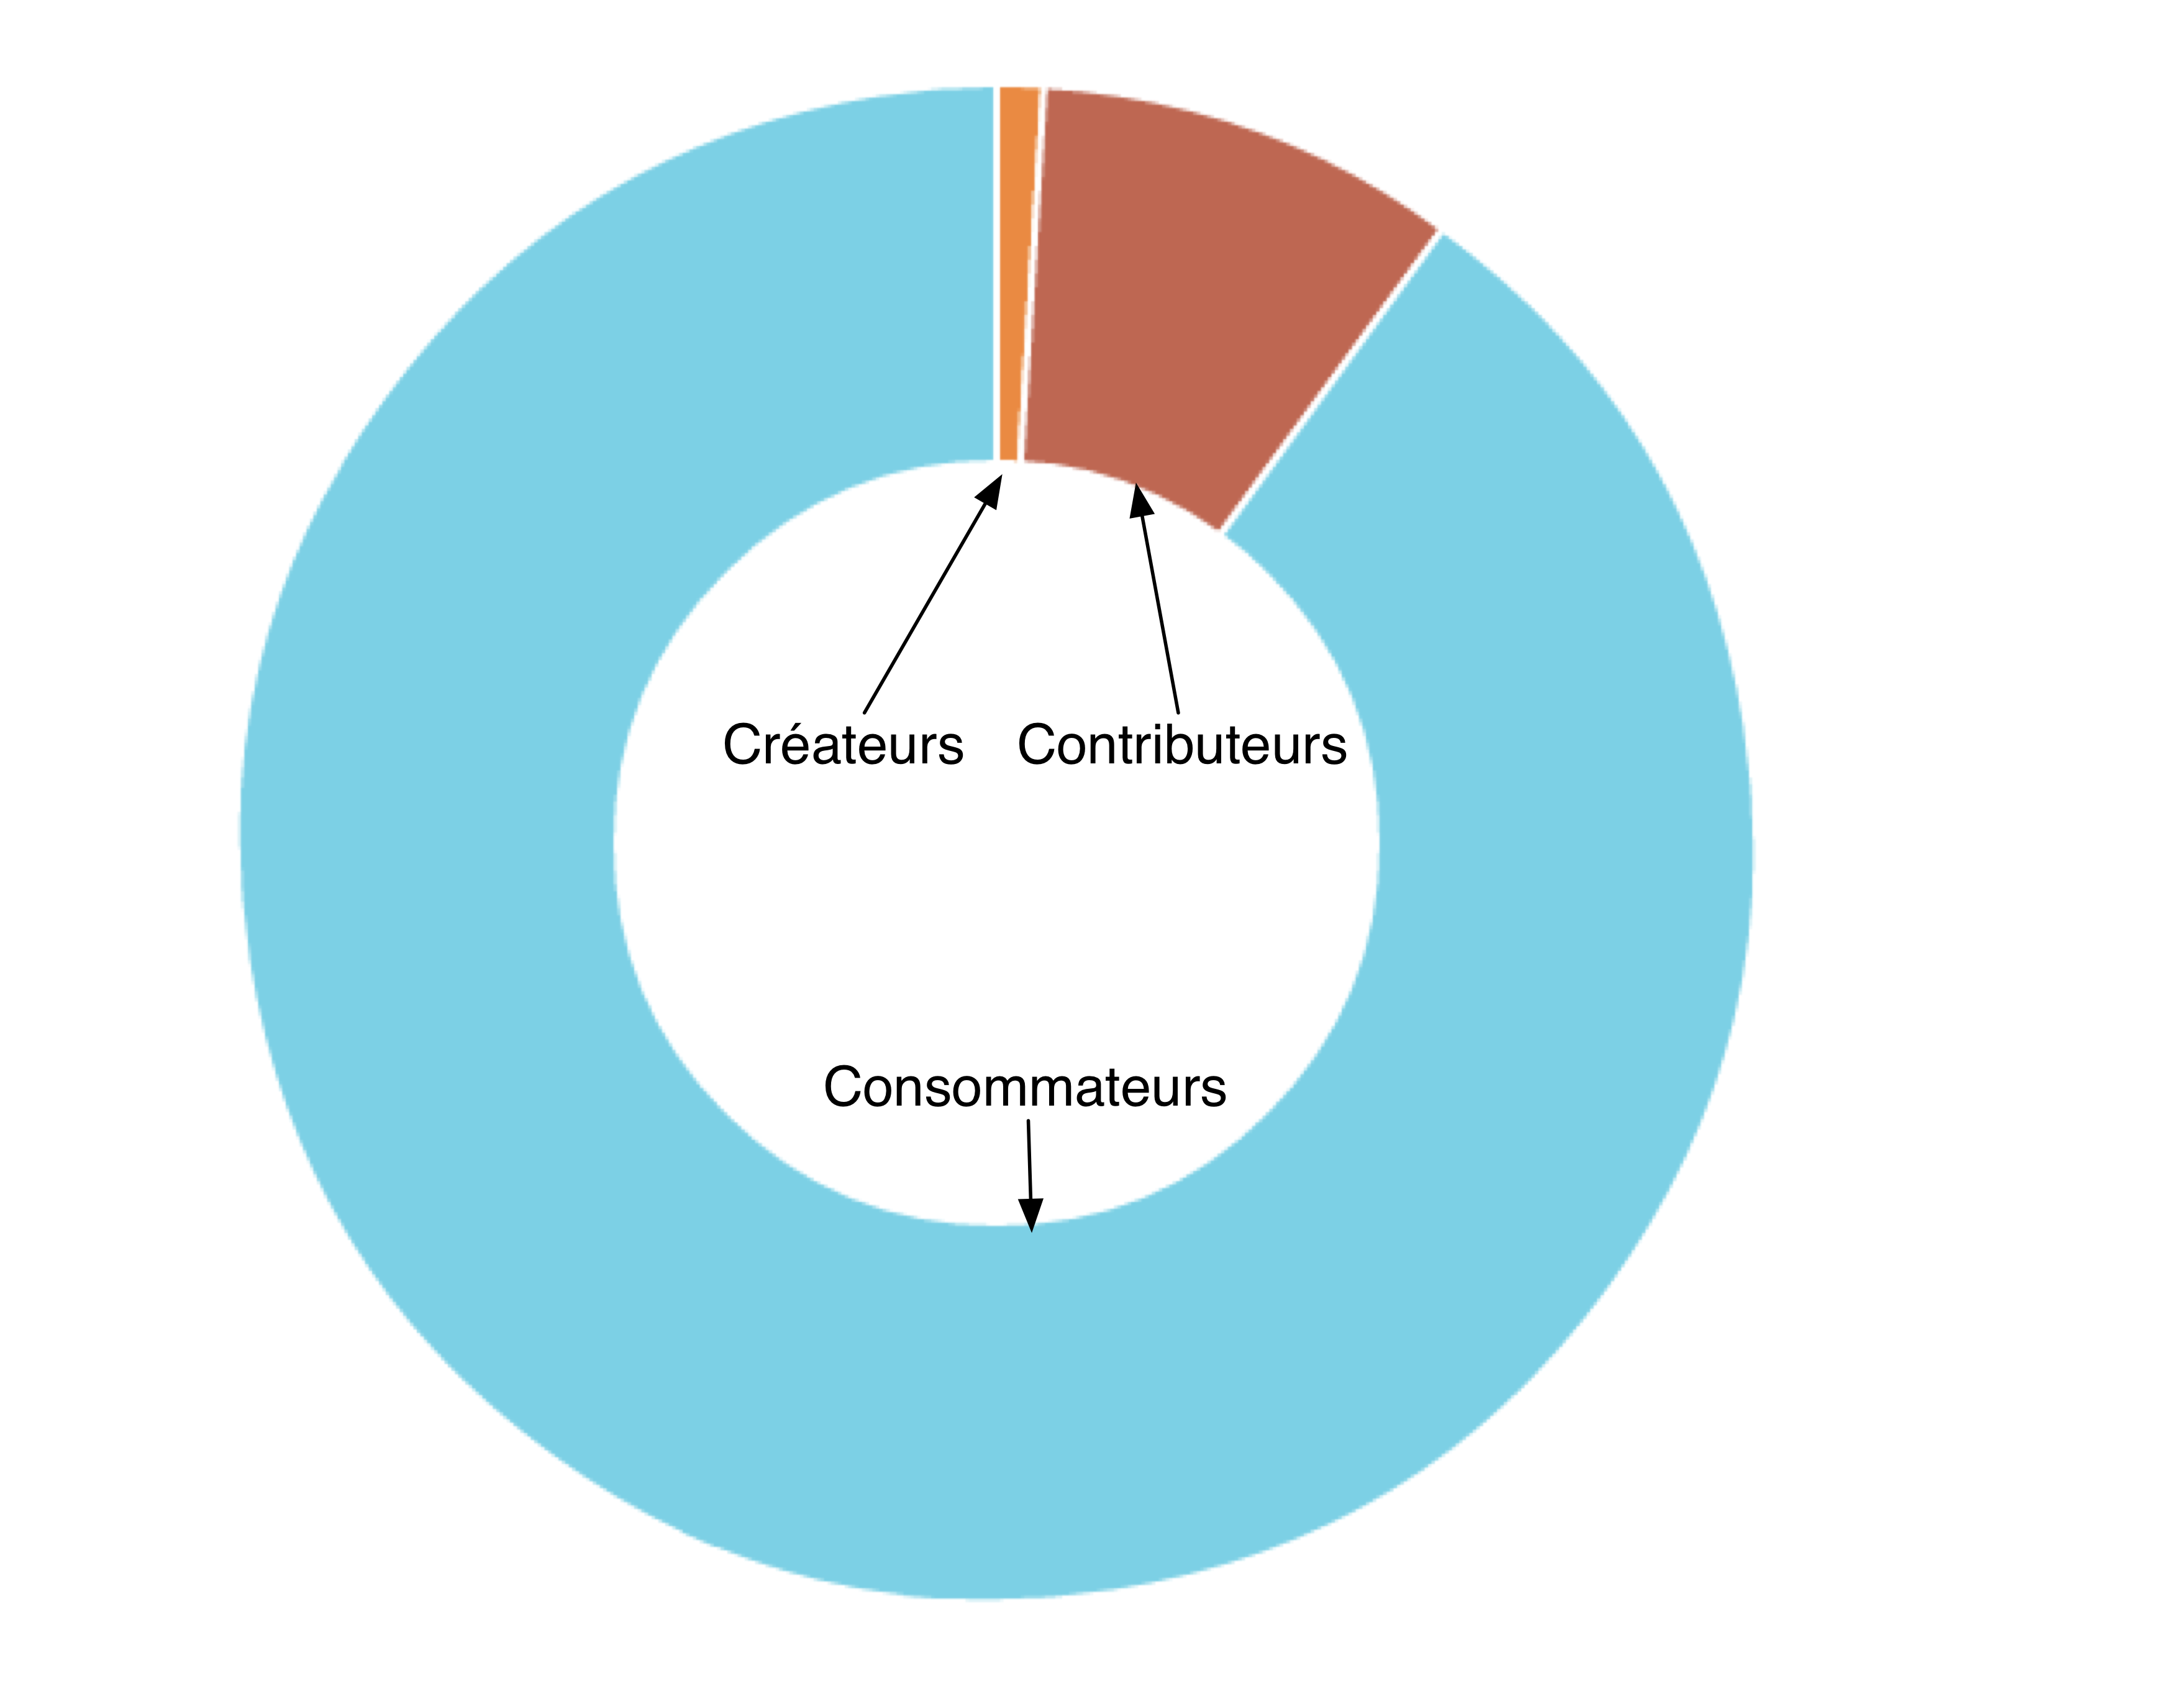
\includegraphics[width=\hsize]{1PercentRule.png}
\caption{1 percent rule}
\end{figure}

\section{Marketing mix}

Pour optimiser la création de valeur et les investissements réalisés sur
nos produits, il est primordial d'adopter un plan marketing. Les
segments clientèle doivent être identifiés et les actions de vente
adaptées.

\subsection{Segments clientèle}

Nous avons étudié en détail les segments de clientèles que nous visons,
en fonction desquels les services et canaux de communications sont
adaptés. L'étude de marché nous permet de cibler trois segments : les
structures à taille humaine, les grandes entreprises et les leaders
d'opinion.

\subsubsection{Petites et moyennes structures}

Le travail d'équipe est bien souvent fondamental dans les PME et
associations ; cependant, la rédaction collaborative de documents autant
que la circulation et l'échange de l'information y sont laborieuses. Par
ailleurs, les e-mails y sont omniprésents et constituent plus une charge
qu'un réel bénéfice pour le salarié. Enfin, ces entreprises n'ont pas de
réelle vocation à maintenir un intranet ou des ressources informatiques
: c'est donc très naturellement que nous leur proposerons notre offre
d'hébergement, de support et de formation, détaillée dans la suite du
présent document.

\subsubsection{Grandes entreprises}

Les points cités précédemment - le travail en équipe et la surcharge
d'e-mails - sont d'autant plus exacerbés dans les grandes entreprises.
En effet, les équipes de travail sont grandes et il est fréquent de
travailler avec des personnes qui ne sont pas côtoyées au quotidien -
contexte international, télétravail, missions. Ainsi, elles mettent
souvent en place des solutions hétérogènes de réseau social d'entreprise
et de rédaction collaborative qui ne répondent pas totalement à leurs
besoins ; elles souhaitent de plus avoir la mainmise sur leurs données
et leur système d'information. Nous leur proposerons donc d'installer
notre produit en leur sein, avec l'appui de leurs équipes IT. Un support
personnalisé leur sera accordé et des formations prodiguées ;
l'intégration avec leurs serveurs d'authentification, de stockage et de
collaboration sera également effectuée.

\subsubsection{Leaders d'opinion}

Nous souhaitons donner la possibilité aux leaders d'opinion de
s'exprimer très facilement sur les sujets qu'ils maîtrisent et qui leur
tiennent à cœur. Ils pourront donc, grâce à notre produit, créer des
communautés rapidement et facilement et partager leur savoir-faire. Les
discussions y seront facilitées et les documents d'importance promus.

L'offre gratuite leur sera accessible, bien que la nécessité de
souscrire un abonnement premium se fasse rapidement sentir. Le coût de
celui-ci peut être supporté intégralement par l'instigateur de la
communauté, mais aussi distribué entre les membres de la communauté.

On peut également ajouter à cette catégorie d'utilisateurs les
chercheurs, qui sont amenés d'une part à rédiger des articles
synthétisant leurs travaux en groupe, et d'autre part à participer à des
sessions de \emph{peer review} - évaluation par les pairs. En effet, ces
usages sont propices à l'édition collaborative, l'apport de corrections,
d'annotations et la création de discussions.

\subsection{Plan marketing}

Notre plan marketing aura pour objectif d'optimiser notre usage des
canaux de communication pour mettre en relation nos services avec nos
segments clientèle.

\subsubsection{Canaux de communication}

Étant donné notre segment clientèle, le plan marketing doit emprunter de
nombreux canaux de communication. Le nombre de ces derniers montrera
aussi l'importance que voue l'entreprise à la promotion de son produit
et sa proximité avec ses clients.

\paragraph{Site Web}

Un site Web sera mis en place pour présenter notre produit. Il
contiendra une présentation du produit à travers un descriptif détaillé,
des captures d'écran et une version de démonstration. Une liste et un
comparatif des services seront tenus et il sera possible de souscrire en
ligne ou de contacter le service commercial. Il permettra aussi de
diffuser les annonces de mises à jour, de modifications ou d'évolutions.
Les informations importantes de l'entreprise seront aussi présentées,
comme l'histoire de l'entreprise, sa politique de confidentialité, ses
éléments d'identification et de contact. Enfin, un blog sera tenu par
l'équipe de développement pour échanger autour des défis techniques
posés par la conception ou l'exploitation, informer des nouveautés ou
des nouveaux employés intégrant l'entreprise. Tous les collaborateurs de
l'équipe seront encouragés à y contribuer pour apporter une pluralité
des points de vue et des expériences, ce qui aura pour effet de
construire et consolider un esprit d'entreprise ainsi que de dresser une
image dynamique et d'accroître notre réputation. Ces articles seront
également l'occasion de mettre en avant les compétences de nos équipes,
leur donner une visibilité et les présenter en autorités dans leurs
domaines respectifs.

\paragraph{Réseaux sociaux}

L'entreprise s'efforcera d'être présente sur les réseaux sociaux -
Twitter, LinkedIn ou Facebook - pour accroitre sa visibilité, donner une
impression de proximité, tenir les utilisateurs au courant d'annonces
importantes ou effectuer du support. C'est une composante très
essentielle de l'image de marque d'une entreprise, où il est très
important de paraître dynamiques et disponibles.

\paragraph{Publicité}

La publicité est historiquement le canal de communication privilégié des
entreprises. Elle permet de toucher un très grand nombre de personnes
dans le cadre de médias de masse en broadcast (télévision, radio, presse
écrite) mais également de cibler son public à l'aide de publicité
contextuelles. C'est cette dernière approche qui est retenue: nous
achèterons des mots clés pour apparaître dans les résultats des moteurs
de recherche ou sur les sites en relation avec notre activité. Des
articles sponsorisés seront aussi achetés, nous permettant de tirer
partie de la crédibilité qu'ont su construire certains blogueurs. Enfin,
les possibilités de mise en avant de nos applications sur les boutiques
d'applications - aussi appelées \emph{stores} ou \emph{markets} -
devront être étudiées.

\paragraph{Conférences et salons professionnels}

Dans une volonté d'être au contact des entreprises, nous participerons à
des conférences d'entreprises sur le travail en équipe et à des salons
professionnels pour présenter notre offre, tels que ceux organisés par
l'ADIM, le MEDEF ou Studyrama. Ces événements desquels raffollent les
\emph{décideurs pressés} sont l'occasion d'entrer en contact direct avec
les personnes ayant le pouvoir d'intégrer nos solutions en entreprise.

L'occasion sera aussi donnée à nos employés de tenir des présentations
lors de conférences - on peut citer Devoxx, PyCon, RTC - pour faire
partager leur connaissances, et augmenter la visibilité et la réputation
de l'entreprise.

\paragraph{Porte-à-porte}

Afin de toucher les grands groupes, notre équipe commerciale devra
démarcher les entreprises pour leur présenter les intérêts et le gain de
notre produit dans le cadre de travail collaboratif. Cette approche
personnalisée permettra de négocier plus aisément des contrats avec ces
entreprises de taille importante. Du matériel promotionnel - plaquettes
commerciales, \emph{goodies} - sera également délivré.

Bien conscients de la difficulté de mener ces actions au début de la vie
d'une start-up, nous envisagerons d'utiliser ce canal de communication
dans un second temps.

\subsubsection{Actions de vente}

Des actions permanentes ou éphémères seront aussi menées pour convaincre
notre cible de recourir à nos solutions.

\paragraph{Version gratuite}

La version gratuite aura pour but, outre d'intégrer de la publicité et
de réunir une communauté d'utilisateurs, de constituer une porte
d'entrée accessible et facile pour faire connaître les avantages de nos
produits. Elle aura ainsi pour vocation de pousser les leaders d'opinion
à souscrire un abonnement payant et d'accroitre l'intérêt des
entreprises.

\paragraph{Campagnes promotionnelles}

Un autre moyen d'attirer les clients est la mise en place de promotions
à l'occasion de divers événements - Noël, anniversaire de la société,
soldes - lors desquels le coût de l'abonnement sera réduit pour une
période temporelle définie. Cependant, ayants confiance en la qualité de
notre produit et en sa réponse à un réel besoin, ce genre d'actions sera
mené avec parcimonie. Nous préférons en effet privilégier les clients
qui nous restent fidèles ou qui représentent un poids financier
important en consentant à des remises commerciales.

\section{Besoins financiers}

Le volet financier constitue un élément important du projet et
déterminera en partie sa réussite future.

Premièrement, des fonds doivent être levés auprès de nos partenaires -
objet du présent cahier. Ces fonds serviront dans un second temps à
soutenir l'envol et l'activité initiale de l'entreprise. Enfin, il nous
faut trouver des solutions pour créer de la valeur \emph{via} la
commercialisation de services à haute valeur ajoutée liés à notre
produit.

\subsection{Sources de financement}

Il nous faut trouver dans un premier temps un fonds financier assez
important pour mener le développement, commencer la commercialisation de
nos services et le marketing associé. Pour cela, les sources sont
multiples et se doivent d'être étudiées en fonction de leur coût :
intérêts, prises de participation, indépendance dans le processus de
décision.

\subsubsection{Apport personnel}

Dans un souci de crédibilité, les créateurs de l'entreprise apporteront
une somme à la hauteur de leur niveau d'investissement dans le projet.
Cet apport personnel déterminera la part de chacun dans le capital de
l'entreprise et la confiance de nos partenaires financier en notre
entreprise sera fonction de ce montant. Un objectif de 20\% du
financement par ce biais semble réaliste et suffisant dans la quête
d'obtention de fonds supplémentaires.

\subsubsection{Fonds d'investissement public}

Il existe également des fonds d'investissements, subventions et
accompagnements au niveau national, régional voire départemental. Ces
organismes publics aident les entreprises qui se créent \emph{via} un
apport financier sans ou avec un très faible taux d'intérêt ou se
portent garant auprès des banques ou des fournisseurs. Ils bénéficient
d'une grande crédibilité et sont des partenaires à ne pas oublier dans
notre recherche de financements. Parmi ces organismes, nous pouvons
citer OSEO, CREALYS et GRAIN en Rhône-Alpes qui financent l'innovation.
Nous avons donc tout intérêt à solliciter au maximum ces organismes pour
diminuer la somme à emprunter auprès d'acteurs privés.

\subsubsection{Capital risque}

Les investisseurs en capital risque - ou \emph{angel investors} - sont
très populaires aux États-Unis dans le soutien de start-ups, en
particulier dans le domaine des technologies de l'information. Google,
Skype ou Dropbox sont des exemples notables d'entreprises ayant suivi
cette voie. Ils apportent leur réseau et leur expérience dans la
création d'entreprises et dans le suivi des premières phases de
développement. Il faut cependant prendre en compte la forte sélectivité
qu'exercent les investisseurs en capital risque, les contraintes de
temps et la prise de participation de ces derniers dans l'entreprise.
Notre objectif consiste donc à lever de 150 000 à 200 000\euro{} pour
financer l'année suivant notre période d'incubation au sein de l'INSA de
Lyon et la mise sur le marché de notre produit.

\subsubsection{Banques}

Les banques sont un partenaire naturel des entrepreneurs pour
l'accompagnement financier de leurs idées, en particulier les banques
d'investissement. Leur aide se fera en fonction de la confiance qu'elles
auront en notre produit, notre \emph{business model} et notre
investissement dans le projet. Leur taux d'intérêts peuvent cependant
être non négligeables et il pourra être très difficile de les convaincre
de s'impliquer dans notre projet. C'est pour cette dernière raison que
le présent cahier est - entre autres - réalisé. Un prêt devra ainsi être
contracté en cas d'échec du financement par des investisseurs en capital
risque. Après la commercialisation de nos services, un rapport étroit
avec les organismes bancaires devra être noué pour financer notre cycle
de production et financer nos investissements futurs.

\subsubsection{Actionnariat}

Une alternative aux investisseurs en capital risque pouvant être étudiée
serait l'ouverture au public du capital de l'entreprise, tout un chacun
prenant des parts dans l'entreprise en échange d'une participation
financière. Des statuts particuliers doivent être considérés pour avoir
la possibilité d'ouvrir le capital et un risque serait pris quant à une
prise de contrôle de l'entreprise par un tiers. Aussi, il faut proposer
une rentabilité financière à court terme pour les actionnaires ce qui
nécessite d'avoir un modèle d'affaires adapté. Cette solution ne sera
envisagée que lors de la viabilité financière de l'entreprise. Ces fonds
seront alors investis dans une structuration plus forte de l'entreprise
et des fonctionnalités toujours plus innovantes et centrées sur les
besoins de nos clients, via une politique forte de recherche et
développement et ainsi capitaliser sur notre expérience.

\subsection{Besoins financiers}

La création d'une start-up dans le domaine de l'ingénierie logicielle
implique des besoins bien particuliers, chiffrés ci-dessous. Le résultat
de cette évaluation des besoins constitue notre objectif pour la
campagne de financement que nous menons. Il faut noter que les montants
ci-dessous sont donnés à titre indicatif et pourront être ajustés. Nous
avons établi un partenariat avec le département
\emph{Télécommunications, Services \& Usages} de l'INSA de Lyon pour
l'incubation durant cinq mois de notre projet. Il en découle des
économies importantes en termes de salaires et d'infrastructures.
Cependant, ce partenariat ne constitue qu'un soutien temporaire et nous
devons par conséquent étudier nos besoins en financement après cette
période d'incubation.

\paragraph{Ressources humaines}

Les hommes et les femmes qui composent nos équipes constituent la force
et le caractère de notre entreprise. Ils sont indispensables dans le
développement et la commercialisation d'un produit de qualité et nous
souhaitons donner une dimension sociale très importante à notre
entreprise.

Durant les premiers mois, le coût de 5 ingénieurs est pris en charge par
l'INSA. Ils devront donc prendre des responsabilités transversales en
sus de la conception du produit.

Ensuite, nous estimons à un chef de projet et deux ingénieurs logiciels
à temps plein les ressources nécessaires au déroulement du projet. Ils
seront épaulés par deux stagiaires. En outre, un commercial sera intégré
à nos équipes pour démarcher des sociétés, organiser des conférences et
participer aux salons d'entreprise. Un chargé de communication qui
prendra également en charge le secrétariat sera lui aussi intégré. Il
s'occupera quant à lui de la création des supports promotionnels, de la
visibilité de nos produit sur l'Internet et participera également aux
salons d'entreprise.

Référence

Heures

Prix unitaire HT

Total HT

Chef de projet

1800

30

54000

Ingénieurs logiciels

3600

30

108000

Commercial

900

25

22500

Chargé de communication

900

20

18000

Stagiaires

3600

10

36000

238500

Dans un premier temps, le chargé de communication et un développeur
seront affectés au support des utilisateurs mais il sera de bon ton
d'engager dès que nos ressources nous le permettront un responsable
qualité ainsi qu'un \emph{Community Manager} pour décharger les
précédents collaborateurs de ce travail qui doit placer le client au
centre de nos préoccupations.

Nous souhaitons de plus nous appuyer sur des fondations solides pour le
développement de notre produit. Ainsi, nous utiliserons des
bibliothèques et des solutions logicielles standard et éprouvées ; nous
privilégierons aussi des bibliothèques \emph{open-source} ce qui nous
permettra de bénéficier de leur communauté d'utilisateurs, leur
réactivité et leur coût négligeable. L'emphase sera alors placée sur les
fonctionnalités du logiciel et leur bénéfice sur les utilisateurs plus
que sur des considérations technico-techniques.

\paragraph{Ressources physiques et organisation}

Dans l'intention de permettre à nos équipes de travailler dans des
conditions optimales, des locaux adaptés à notre activité sont
nécessaires. Ils devront proposer un \emph{open-space}, une salle de
conférence et un espace de détente. Des bureaux individuels ne semblent
pas nécessaires étant donné le faible nombre d'employés composant
l'entreprise mais aussi pour limiter la distribution des pouvoirs - une
mesure de l'importance de la hiérarchie dans les relations entre les
employés. Des équipements informatiques sont indispensables considérant
le monde numérique d'aujourd'hui et le secteur d'activité dans lequel
nous opérons. De plus, un ordinateur sera affecté à chacun des employés
qui en fera la demande et ils pourront demander tout équipement
nécessaire à leur activité (serveurs, écrans, périphériques, pièces
détachées\ldots{}) ; aussi, nous accorderons le droit à nos équipes
d'utiliser leur propre matériel s'ils le désirent. Les fournitures de
bureau standard seront enfin en libre accès.

Une connexion à Internet est également indispensable pour la conduite de
notre activité.

Pour la version en ligne de notre produit, nous ferons appel à un
prestataire de stockage dans le \emph{cloud}. Cette solution représente
l'avantage d'être flexible et s'adaptera ainsi à la croissance de
l'utilisation du produit. De plus, cela offre le confort d'une
maintenance externalisée et et de tarifs avantageux. Amazon Web Services
est un acteur majeur du stockage et de l'hébergement dans le cloud et
reconnu par tous par sa fiabilité, sa fiabilité et son support.

Référence

Coût annuel HT

Bureaux

36000

Matériel informatique

10000

Fournitures de bureau

200

Connexion à Internet

600

Abonnements téléphonie mobile

1500

Infrastructure d'hébergement

f(nombre d'utilisateurs)

48300 + f(nombre d'utilisateurs)

où f(nombre d'utilisateurs) \textasciitilde{}= nombre d'utilisateurs *
2\euro{} / mois

On pourrait également considérer, au moins pour une partie, le coût de
l'infrastructure pour les utilisateurs d'une offre gratuite comme une
charge de publicité. Tous ces coûts seront nuls au cours des cinq
premiers mois grâce à notre partenariat. Des actions auprès de
l'Institut National de la Propriété Intellectuelle sont aussi à mener
pour protéger notre marque, notre logo et notre produit. Si notre
activité prend une dimension internationale importante, ces mêmes
actions devront être portées auprès des bureaux de propriété
intellectuelle étrangers, où nous devrons aussi déposer nos savoir-faire
dans le cas où les brevets logiciels seraient reconnus.

\paragraph{Marketing}

Le marketing, bien qu'espoir de retombées économiques, a un coût qu'il
faut prendre en compte. Il se traduit par la création et l'hébergement
d'un site Web, la création de vidéos ou de supports de présentation. Ces
actions seront menées après la période d'incubation, dès lors que nous
aurons un produit à la hauteur des attentes du client. La participation
aux conférences et salons d'entreprises représente également un coût,
justifié par l'occasion de rencontrer directement les professionnels
constituant l'un de nos segments clientèle et de procéder à un aperçu
des bénéfices qu'ils pourraient tirer de l'utilisation de notre produit.
Ce type d'événement concède un retour sur investissement très important
et permet d'établir une proximité forte avec les professionnels et de
donner une visibilité importante sur notre marque et nos solutions.

Référence

Prix HT

Hébergement

1000

Nom de domaine

15

Vidéos

2000

Flyers

1000

Présentations

500

Conférences

10000

14515

\subsection{Commercialisation}

La commercialisation de notre produit, et ainsi la création de valeur,
est une dimension très importante de notre projet dans la mesure où elle
permettra de valider le travail de notre équipe. Les orientations ou les
choix techniques devront donc être pris et affinés en adéquation avec
nos objectifs. Les différents services proposés par notre société
s'inspirent sur ce qui a fait et continue de faire la réussite de
nombreux acteurs de l'informatique, et plus particulièrement du Web.
Enfin, nos offres correspondent aux segments de marché visés et placent
les intérêts de nos clients en haut lieu.

\subsubsection{Version basique}

Une version gratuite en ligne sera proposée pour permettre à l'ensemble
des utilisateurs de connaître notre produit, ses caractéristiques et ses
atouts. Elle sera dotée des fonctionnalités standard telles que la
discussion ou l'édition de documents qui font la force et l'intérêt de
notre produit. Cependant, cette version sera amputée de l'édition
collaborative en temps réel ou de la gestion fine des permissions. La
version basique cible les leaders d'opinion qui souhaitent monter une
communauté bâtie autour du même centre d'intérêt. De la publicité sera
en outre intégrée ; il est en effet essentiel de monétiser chaque
utilisateur et une hausse de la base d'utilisateurs doit entraîner
mécaniquement une hausse de nos revenus, que ce soit par une
augmentation des souscriptions à nos services payants ou par des revenus
publicitaires plus importants. En outre, l'intégration de tels encarts
permettra de supporter les coûts de stockage associés.

\subsubsection{Version premium}

Apportant des fonctionnalités telles que l'édition collaborative en
temps réel, la gestion fine des permissions, la visibilité des contenus
ou le choix de formats d'export, cette version ciblera les petites et
moyennes entreprises ainsi que les associations n'ayant pas les
ressources temporelles ou financières de gérer un intranet ou un
ensemble d'applicatifs métier supportant leurs activités. En effet,
l'hébergement et la maintenance seront assurés par nos soins, les
déchargeants de ces opérations dans un but de rationalisation des coûts.
De plus, l'interface sera débarrassée des publicités et le nom de
domaine sera personnalisable.

En l'échange d'un abonnement mensuel ou annuel - à ce dernier étant
associé une remise pour fidéliser nos clients - sera accordé l'usage de
la plate-forme à un ensemble de personnes appartenant à l'organisation.
Aussi, le client bénéficiera des mises à jour qui seront déployées et
d'un support en ligne réactif. Le tarif sera également fonction du
nombre d'utilisateurs concernés.

\paragraph{Étudiants}

Les étudiants pourront quant à eux bénéficier de cette version premium
gratuitement dans le cadre de notre engagement fort en faveur de
l'éducation. Leurs projets scolaires pourraient ainsi être réalisés à
l'aide de notre produit. Cette version constituera un vecteur marketing
très important en exploitant les techniques dites de l'appât et de
l'hameçon : l'objectif est de sensibiliser, convaincre et fidéliser
cette clientèle qui deviendra les décideurs de demain.

\subsubsection{Version entreprise}

Les grandes entreprises sont ici visées par cette version, reprenant
l'ensemble des fonctionnalités premium. Cette version se démarque par
l'installation de la plate-forme au sein des infrastructures du client
en collaboration avec ses équipes IT. Un support avancé sera offert pour
l'intégration du produit avec les serveurs d'authentification ou de
collaboration en place. La souscription à ce service se fera \emph{via}
un abonnement mensuel ou annuel.

\subsubsection{Support}

Le support constitue un atout majeur dans le domaine de l'ingénierie
logicielle. Des équipes de support courtoises et performantes rassurent
le client et influent grandement dans le processus de vente d'un produit
ou d'un service. Il est en effet essentiel pour un client, en
particulier une grande entreprise dont le logiciel en question est un
élément essentiel de son \emph{workflow}, d'avoir un interlocuteur en
cas de difficulté lors de l'utilisation du logiciel ou si il est victime
d'un éventuel bug ou dysfonctionnement du logiciel. Ce dernier cas est
très intéressant pour l'accroissement de la qualité du logiciel et il
est de ce fait très important que le problème soit remonté aux
développeurs. C'est pourquoi la relation client est une composante à
part entière des services que nous proposons.

Dans le cadre de la version gratuite, ce support se fera principalement
par mail par nos équipes, mais nous mettrons aussi en place un forum et
un salon de discussions pour permettre une entraide par la communauté.
Lors de la souscription à l'un de nos services, le client aura quant à
lui un accès par téléphone au support et aura la garantie d'une réponse
sous deux jours ouvrés.

En sus de l'argument de vente et de l'élimination de potentiels
\emph{bugs}, le support peut être générateur direct de ressources et
nous proposerons des contrats de support personnalisés, offrant une
priorisation des recours au support, une garantie de temps de
rétablissement, des formations ou l'implémentation de fonctionnalités.

\subsubsection{Récapitulatif des offres}

Les offres proposées et leur prix associé sont synthétisés dans le
tableau ci-dessous.

Produit

Basique

Premium

Entreprise

Frais initiaux

offerts

offerts

2000\euro{}

Abonnement

0\euro{} mais publicité (\textasciitilde{}2\euro{}/utilisateur/mois)

40\euro{}/groupe/mois ou 5\euro{}/utilisateur/mois

20\euro{}/utilisateur/mois

Support

inclus (communauté)

inclus (sous 48h)

à partir de 1000\euro{}/mois

Rentabilité

∞

600 groupes

300 entreprises

\begin{center}
\begin{tabularx}{\hsize}{|c|c|c|c|}
  \hline
Produit & Basique & Premium & Enterprise \\
  \hline
Frais initiaux & offerts & offerts & 2000\euro \\
  \hline
\end{tabularx}
\end{center}

Notre objectif est de toucher tous les créateurs de contenus à forte
valeur ajoutée en leur proposant des offres adaptées à leur besoin pour
leur faciliter la création de valeur.

\section{Management de projet}

\subsection{Présentation de l'équipe}

Notre équipe est composée de futurs ingénieurs de l'INSA de Lyon, du
département Télécommunications, Services \& Usages, partageant une
motivation commune autour de ce projet.

Voici les différents membres de l'équipe :

\begin{itemize}
\itemsep1pt\parskip0pt\parsep0pt
\item
  Guillaume Burel ;
\item
  Xiao Yu Feng ;
\item
  Fabio Guigou ;
\item
  Baptiste Metge ;
\item
  Paul Mougel : chef de projet.
\end{itemize}

\subsection{Fonctionnement de l'équipe}

Il convient de définir une organisation commune permettant de respecter
les délais impartis tout en menant à bien le projet. Suivant les
conseils de nos tuteurs, nous avons tout d'abord rédigé une charte
consignant les règles de fonctionnement interne qui devront être suivies
par les membres de l'équipe tout au long du projet.

Le chef de projet a notamment pour charge de coordonner les membres de
l'équipe et de s'assurer de la validité des différents livrables ainsi
que du respect des dates butoirs.

\textbf{Prises de décisions} L'équipe étant animée d'une même volonté,
nous avons décidé de prendre autant que possible l'ensemble des
décisions de manière collégiale. En cas de problème majeur, la décision
revient au seul chef de projet.

\textbf{Réunions de travail} Chaque réunion de travail est accompagnée
d'un ordre du jour précis listant le temps alloué pour chaque point à
traiter. Chaque réunion se conclut par un bref résumé oral et la
rédaction d'une liste des tâches à réaliser avant la prochaine réunion
pour chaque membre de l'équipe. Nous nous réunirons une fois par semaine
au minimum.

\textbf{Documentation} Chaque réunion fait l'objet d'un compte-rendu
dont la responsabilité incombe au secrétaire de séance. Nous disposons
également d'un wiki interne où chaque membre documente son travail ;
chacun peut alors se familiariser avec les technologies et les problèmes
spécifiques rencontrés. Ce wiki a pour vocation de se transformer en
véritable base de connaissances au fil de l'avancement du projet.

\textbf{Outils} Nous utilisons le service d'hébergement et de gestion de
développement de logiciels GitHub. Cet outil permet à chacun de suivre
l'avancement du projet en ayant une vue d'ensemble claire des tâches à
réaliser et des problèmes à corriger.

\textbf{Développement} Durant la phase II, l'équipe s'organisera autant
que possible selon les préceptes agiles, tels qu'un fonctionnement
itératif cyclique organisé en sprints.

\section{Licence}

\subsection{Choix de la licence}

Notre produit sera distribué sous une \textbf{licence propriétaire}. En
effet, nous n'avons pour l'instant aucun avantage à ouvrir les sources :
nous n'aurons aucun contributeur extérieur avant que le projet ait
atteint un certain stade de maturation. Ainsi, il est pour l'instant
préférable de garder un contrôle complet de notre projet. Par ailleurs,
il est plus facile de vendre un produit qui n'est pas accessible au
grand public ; en particulier, le serveur et la base de données n'ont
aucune raison d'être rendus publics. Un passage à l'\emph{open source}
peut par la suite être envisagé si le besoin d'une communauté se fait
sentir, par exemple pour l'écriture de modules additionnels.

\subsection{Contraintes}

L'utilisation d'une licence propriétaire a des conséquences au niveau
des bibliothèques utilisables pour la réalisation du projet. Certaines
licences libres, en particulier GPL, sont "contaminantes" : tout
projet les incluant doit être distribué sous la même licence. Nous
devrons donc nous limiter à des licences moins restrictives comme
Apache, MIT ou BSD. Heureusement, le nombre de projets \emph{open
source} utilisant de telles licences est assez élevé pour que notre
développement ne soit pas entravé par un manque de code disponible. \#
Analyse des risques

Toute activité industrielle conduit à l'apparition de phénomènes
inattendus qui doivent être étudiés en amont. Aussi, ils doivent faire
l'objet de procédures drastiques pour réagir de manière adéquate. Il est
illusoire d'espérer être parés à toutes ces situations : c'est pour cela
que chaque situation sera consignée dans un document dédié et conduira à
la rédaction d'un rapport listant les actions à mener pour empêcher sa
réapparition dans le futur ou en limiter les conséquences.

\subsection{Risques liés au produit}

Nous listons ici la plupart des risques opérationnels liés à la
livraison et l'exploitation de notre produit, pouvant attiser
l'incompréhension voir la colère de nos utilisateurs.

\begin{itemize}
\itemsep1pt\parskip0pt\parsep0pt
\item
  \emph{panne de l'offre cloud} : il nous faudra renégocier des contrats
  avec notre partenaire afin d'augmenter la redondance et de diminuer la
  garantie de temps de rétablissement (GTR). Il sera également
  envisageable de recopier automatiquement les données chez plusieurs
  hébergeurs, bien que cela implique un temps de développement et de
  maintenance accru. Nous effectuerons de plus un geste commercial
  envers les utilisateurs payants afin de les dédommager pour
  l'indisponibilité de l'outil. Ce risque est qualifié de peu critique
  si la durée d'indisponibilité est limitée.
\item
  \emph{perte de données} : très critique, ils nous faut limiter cette
  éventualité dans la mesure du possible par la mise en place en amont
  de sauvegardes automatiques.
\item
  \emph{non satisfaction des clients} : pouvant mettre en péril notre
  société, ce risque est considéré comme critique. Afin de recueillir
  les commentaires de nos clients, nous mettrons en place une
  plate-forme de suggestions, contacterons personnellement les clients
  les plus importants voire engagerons un consultant afin de nous
  recentrer sur les fonctionnalités cœur. Un renfort des équipes support
  et marketing sera également à envisager.
\item
  \emph{concurrence} : notre produit évoluant dans un secteur
  concurrentiel, il nous faudra surveiller attentivement l'évolution des
  solutions concurrentes afin d'évaluer plus précisément les risques
  posés par chaque compétiteur.
\item
  \emph{bug logiciel} : l'ingénierie logicielle n'étant pas une science
  exacte, il est envisageable que notre produit comporte des bugs. Ce
  risque sera très présent tout au long de la vie de notre société et
  devra être contenu à travers la mise en place d'une démarche qualité
  et d'une politique de tests approfondis.
\item
  \emph{mauvais choix de technologies} : peu critique au regard des
  clients de notre société pour lesquels la technologie utilisée n'a que
  peu d'impact, un mauvais choix technologique limitera fortement notre
  vélocité de développement ainsi que notre capacité à faire évoluer
  notre produit. Il sera crucial d'évaluer les technologies choisies
  avant de commencer la phase de développement du produit. Nous
  instaurerons également une veille technologique qui aura pour but de
  surveiller l'état de l'art et qui nous permettra d'évaluer rapidement
  les alternatives possibles si les limitations de certains de nos
  outils se font sentir.
\end{itemize}

\subsection{Risques humains}

Dans cette section sont listés les risques liés à la composante humaine
de notre projet.

\begin{itemize}
\itemsep1pt\parskip0pt\parsep0pt
\item
  \emph{équipe peu productive ou démotivée} : ce risque est critique et
  deviendra de plus en plus présent au fur et à mesure de l'avancement
  du projet. Il nous faudra alors nous concentrer sur l'essentiel des
  fonctionnalités ou revoir nous objectifs à la baisse. Nous
  envisagerons également d'engager du personnel supplémentaire tel que
  des consultants ou des stagiaires qui apporteront leur point de vue
  neuf sur notre projet.
\item
  \emph{deadline non respectée} : ce risque est important et sera
  atténué par une organisation agile, centrée sur des \emph{sprints} de
  développements courts, nous permettant ainsi une évaluation rapide de
  nos performances.
\end{itemize}

\subsection{Risque financiers}

Enfin, il convient d'analyser les risques posés par le volet financier
de notre projet.

\begin{itemize}
\itemsep1pt\parskip0pt\parsep0pt
\item
  \emph{financement non suffisant} : très critique, un financement
  insuffisant impacterait fortement notre capacité à mener à bien notre
  projet. Nous envisagerons alors de faire appel à des investisseurs en
  capital risque ou à des \emph{business angels} qui prendront alors une
  part de participation dans notre société.
\item
  \emph{frais trop importants par rapport aux ressources} : risque
  critique et difficile à évaluer au démarrage de notre activité, il
  nous faudra surveiller attentivement nos dépenses afin que nos frais
  soient en adéquation avec les profits effectués par notre entreprise.
\item
  \emph{mauvais positionnement tarifaire}, qui peut impliquer deux
  possibilités 1) des clients présents mais trop peu rentables 2) trop
  peu de clients du fait d'un prix demandé trop élevé. Une étude poussée
  des solutions concurrentes nous aidera à nous positionner au lancement
  de notre produit. Nous envisagerons également d'engager un consultant
  afin d'étudier le positionnement tarifaire de notre offre.
\item
  \emph{trop peu de ressources} : il conviendra dans ce cas de
  ré-étudier le plan marketing ou de se concentrer sur un segment
  clientèle plus restreint afin de proposer un produit plus ciblé.
\end{itemize}

\section{Évolutions possibles à long terme}

Cette partie constitue une réflexion sur les évolutions possibles de
notre outil dans un futur plus lointain. Bien que nous souhaitions pour
l'instant nous concentrer sur les fonctionnalités cœur il semble
important de proposer quelques perspectives d'avenir. En voici une liste
non exhaustive.

\subsection{Application pour smartphone}

Une évolution vers une plate-forme mobile est incontournable de nos
jours. Bien que la rédaction soit plus agréable sur un ordinateur
classique, offrir à nos clients la possibilité de visualiser leurs
documents depuis un terminal mobile est très important.

\subsection{Socialisation}

Apporter une dimension sociale est importante pour offrir une
plate-forme de travail virtuel vivante et agréable. Cela peut passer par
des pages de profils présentant les travaux réalisés par un utilisateur
et la mise en contact de personnes ayant des intérêts communs.

\subsection{Orientation scientifique}

Notre outil peut permettre la rédaction d'articles scientifiques et la
mise en contact de chercheurs. Si cette orientation est choisie, il nous
faudra adapter notre outil à la rédaction scientifique en proposant une
gestion des formats utilisés fréquemment par la communauté scientifique,
notamment LaTeX. Une équipe de chercheurs pourra alors utiliser notre
outil afin de préparer la rédaction d'un article tout en prenant en
compte les commentaires de différents relecteurs.

\subsection{Importation de documents externes}

Pouvoir importer un document externe de type PDF pour ensuite partager
une discussion sur celui-ci peut être une évolution possible. Cela
permettrait de profiter de l'interface de discussion de notre outil,
même si le document n'en est pas originaire.

\section{Découpage en lots}

La phase de réalisation du projet est découpée en plusieurs sous-parties
appelées \emph{lots}. La réalisation de chaque lot se conclut par la
livraison d'une partie pleinement utilisable du projet et par une phase
de tests, effectuée à la fois par l'équipe mais aussi par des
intervenants extérieurs, permettant d'analyser la pertinence du
développement et des orientations prises par l'équipe.

Afin que ce découpage en lots soit pertinent, nous avons cherché à
isoler les différentes composantes du projet, listées dans le graphique
ci-dessous.

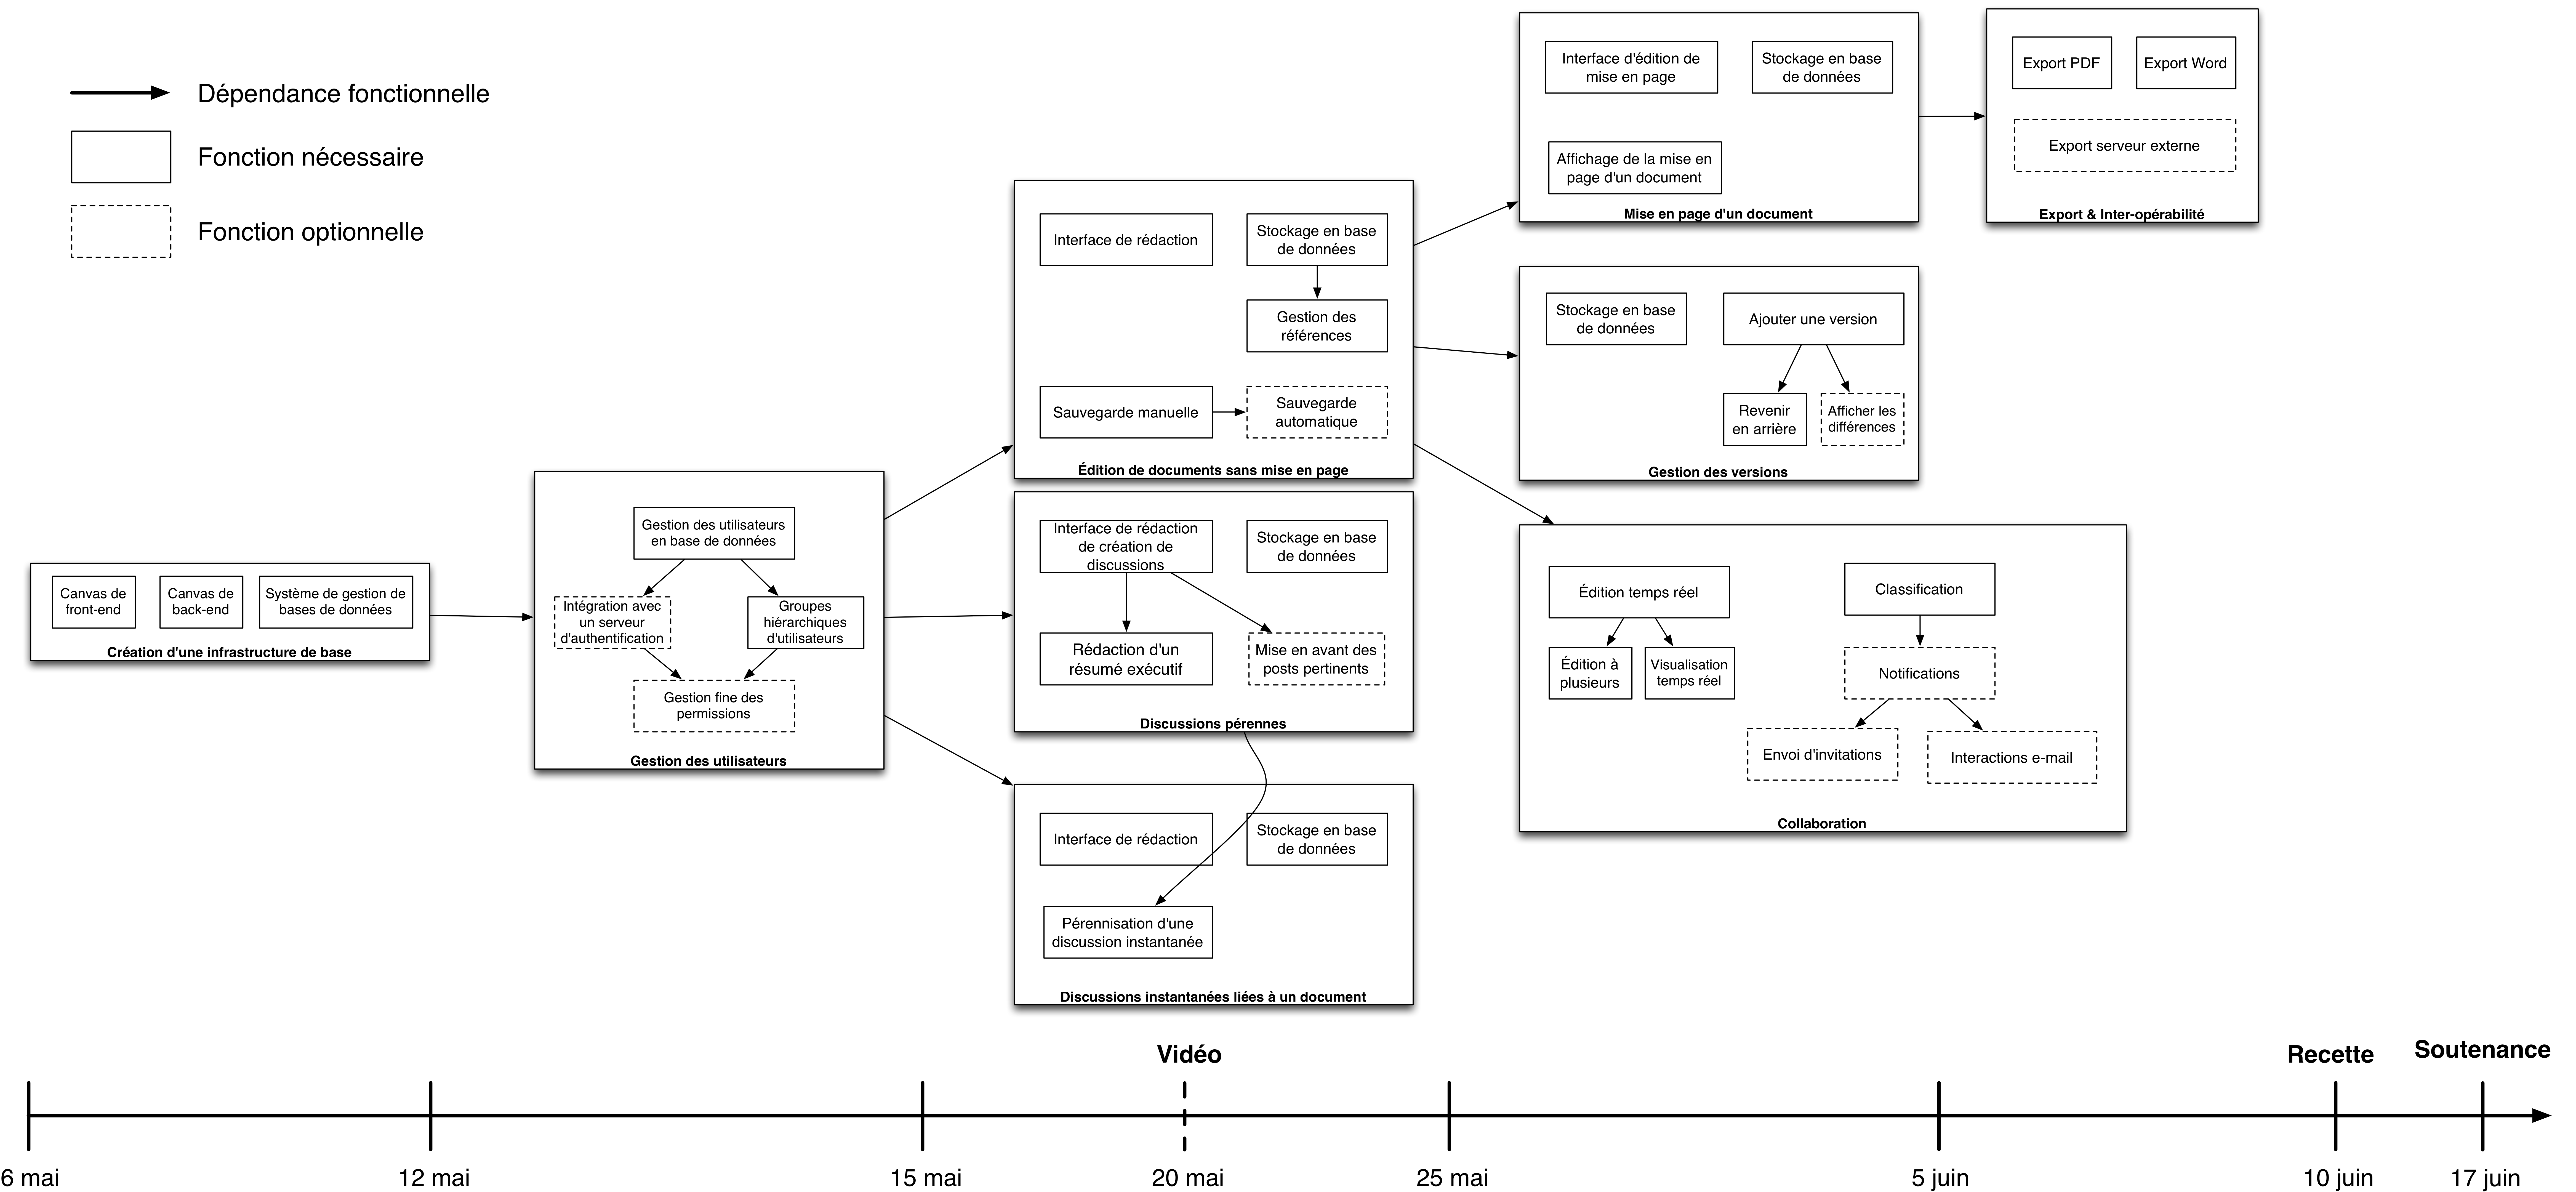
\includegraphics[width=\linewidth,height=\textheight,keepaspectratio]{pert.png} 

\section{Liste des fonctionnalités}
Nous listons dans cette annexe les fonctionnalités que notre produit
devra offrir dans une version plus aboutie que le premier prototype qui
sera développé d'ici la fin de la phase II.

\subsection{Document}

\begin{itemize}
\itemsep1pt\parskip0pt\parsep0pt
\item
  Rédaction simple et intuitive de documents structurés
\item
  Sauvegarde automatique des documents en cours de manipulation par
  l'utilisateur
\item
  Édition d'un même document par plusieurs personnes de manière
  simultanée
\item
  Affichage des ajouts, modifications et suppressions d'un document par
  des collaborateurs en temps réel
\item
  Export d'un document dans un format standard et pérenne (tel que le
  PDF)
\item
  Export d'un document vers un serveur de collaboration ou de stockage
\item
  Export d'un document dans un format éditable (tel que le \emph{docx})
\item
  Sélection de feuilles de styles pour l'export des documents
\end{itemize}

\subsection{Collaboration}

\begin{itemize}
\itemsep1pt\parskip0pt\parsep0pt
\item
  Création de discussions autour d'un document
\item
  Invitation d'un collaborateur à rejoindre une discussion (\emph{via}
  \textbf{@}user)
\item
  Rédaction d'un document de manière collaborative
\item
  Notification de l'évolution d'un document ou d'une discussion (par
  e-mail, SMS)
\item
  Annotation aisée et précise d'un document collaboratif
\item
  Pérennisation d'une discussion instantanée en un fil de discussion
\item
  Clore une discussion en la résumant
\item
  Intégration et interaction des e-mails dans les discussions
\item
  Export et synchronisation d'une discussion avec un ou plusieurs
  services externes (réseau social, Q\&R, etc.)
\item
  Référence simple d'une ressource depuis une discussion ou un document
  (\emph{via} \textbf{\^{}}document)
\item
  Stockage différentiel des versions d'un document
\item
  Visualisation de l'historique des modifications d'un document
\item
  Restauration d'une version quelconque d'un document avec conservation
  de l'historique des modifications
\item
  Création de versions concurrentes et parallèles d'un document
\item
  Catégorisation des documents et discussions, afin de permettre une
  recherche aisée
\item
  Promotion des documents importants
\item
  Promotion des posts intéressants
\item
  Intégration de dates butoir dans le processus de rédaction d'un
  document
\item
  Possibilité pour l'administrateur d'un document de protéger son
  édition pour relecture, validation et commentaires
\item
  Disponibilité d'un mode zen (ou \emph{ne pas déranger}) pour maximiser
  l'efficacité de l'utilisateur lors de la phase de rédaction
\end{itemize}

\subsection{Simplicité}

\begin{itemize}
\itemsep1pt\parskip0pt\parsep0pt
\item
  Interface épurée, réactive, \emph{responsive} et dotée de peu
  d'options
\item
  Présence d'un guide de démarrage (animation, vidéo, FAQ)
\item
  Compatibilité du produit avec la majorité des navigateurs respectant
  les standards du Web
\end{itemize}

\subsection{Autres}

\begin{itemize}
\itemsep1pt\parskip0pt\parsep0pt
\item
  Création et gestion de groupes d'utilisateurs associés à des
  permissions
\item
  Gestion de la visibilité d'un contenu
\item
  Intégration à un serveur d'authentification
\end{itemize}

\section{Business Model Canvas}

\begin{figure}[htbp]
\centering
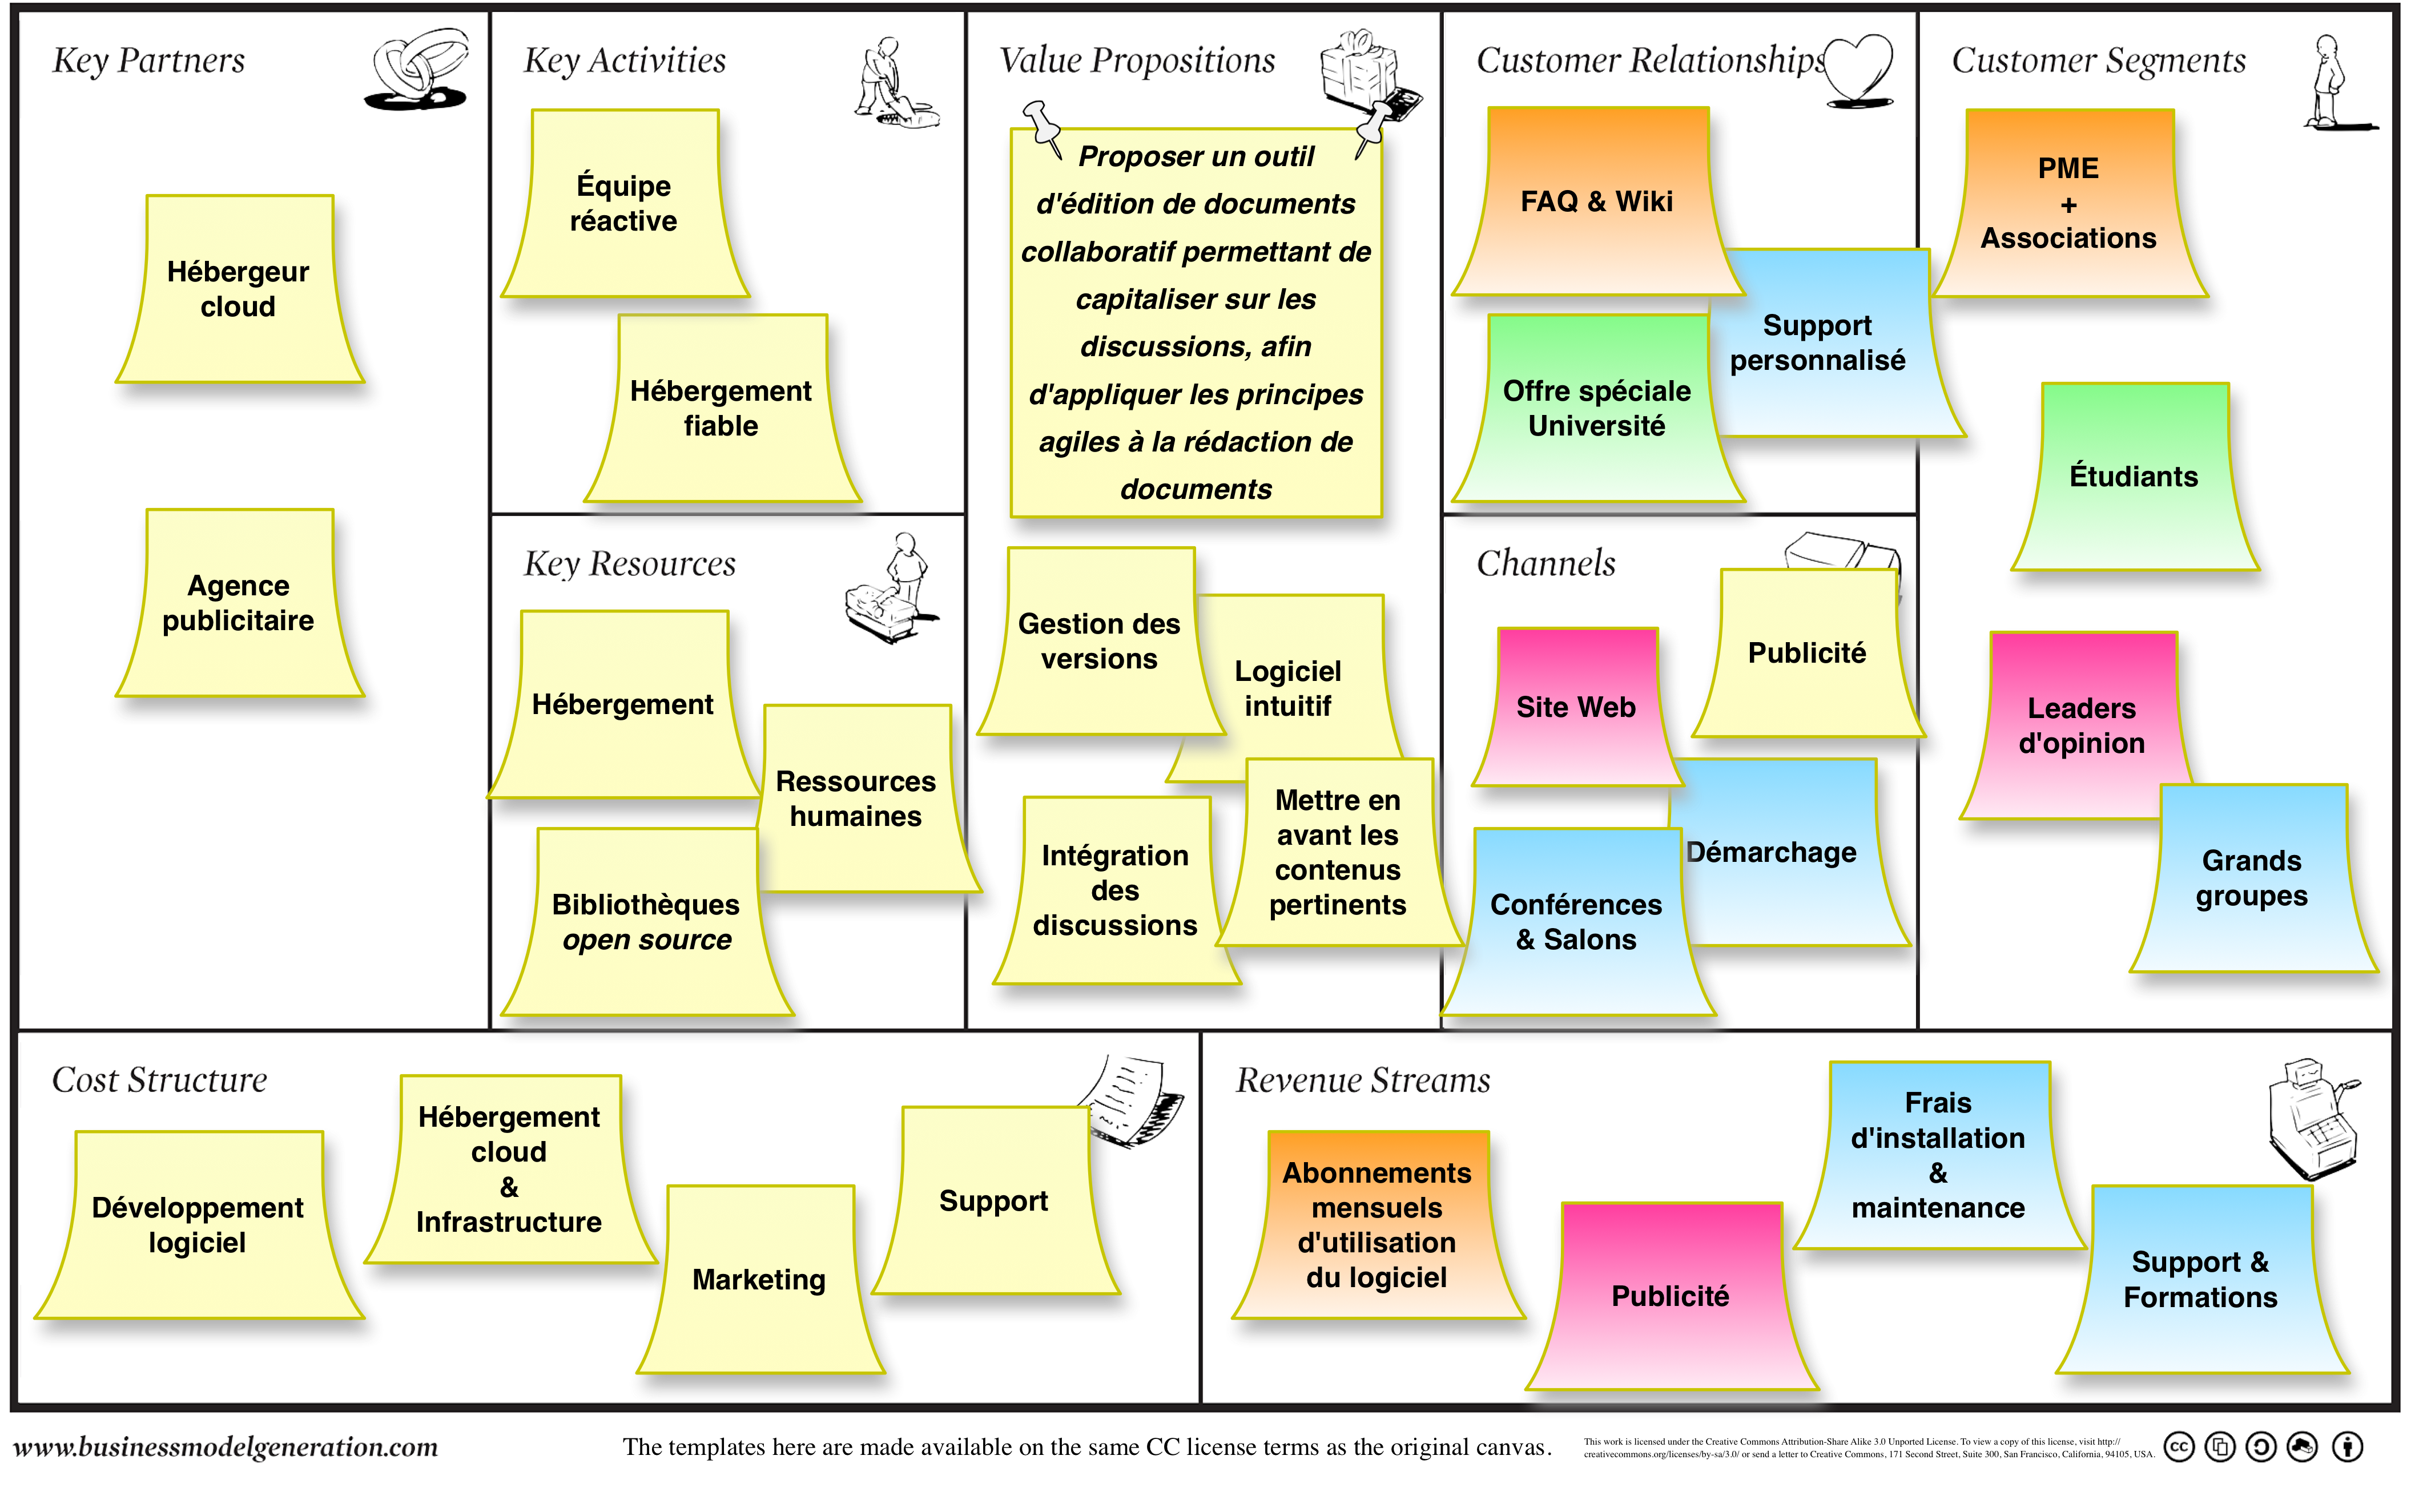
\includegraphics[width=\hsize]{business_model_canvas.png}
\end{figure}

%\end{multicols}
\end{document}

